\documentclass{jcst}
\usepackage[utf8]{inputenc}
\usepackage[T1]{fontenc}
\usepackage{float}
\usepackage{balance} % balances the columns of the last page (flushend does not manage it with the citation box)

\graphicspath{{figures/}}

% TikZ figures
\usetikzlibrary{positioning,arrows.meta,fit,backgrounds,calc}
\definecolor{vendorfill}{HTML}{EAF1FB}
\definecolor{vendornode}{HTML}{D5E3F7}
\definecolor{vendorline}{HTML}{5B7DB1}
\definecolor{custfill}{HTML}{FFF8E6}
\definecolor{custnode}{HTML}{FBE9C2}
\definecolor{custline}{HTML}{C99A2E}
\definecolor{l1fill}{HTML}{FCE4EC}
\definecolor{l1line}{HTML}{C2185B}
\definecolor{l2fill}{HTML}{FFF3E0}
\definecolor{l2line}{HTML}{EF6C00}
\definecolor{l3fill}{HTML}{FFFDE7}
\definecolor{l3line}{HTML}{B59B00}
\definecolor{l4fill}{HTML}{E3F2FD}
\definecolor{l4line}{HTML}{1565C0}
\definecolor{llmfill}{HTML}{EDE7F6}
\definecolor{llmline}{HTML}{6A4C9C}
\definecolor{hardfill}{HTML}{F3E5F5}
\definecolor{hardline}{HTML}{8E24AA}
\definecolor{failfill}{HTML}{F8D7DA}
\definecolor{failline}{HTML}{B71C1C}
\definecolor{okfill}{HTML}{E6F4EA}
\definecolor{okline}{HTML}{2E7D32}
\definecolor{outblock}{HTML}{B03A2E}
\definecolor{outtrace}{HTML}{7D3C98}

% Float placement: let pages carry more floats so that the result tables of
% Section 7 stay close to their text instead of drifting past the back matter.
\renewcommand{\topfraction}{0.95}
\renewcommand{\bottomfraction}{0.6}
\renewcommand{\textfraction}{0.05}
\renewcommand{\floatpagefraction}{0.75}
\renewcommand{\dbltopfraction}{0.95}
\renewcommand{\dblfloatpagefraction}{0.75}
\setcounter{topnumber}{3}
\setcounter{totalnumber}{5}
\setcounter{dbltopnumber}{1} % never stack two double-column floats on one page

% Markers for content that depends on the pending experimental campaign.
\newcommand{\TBD}{\textbf{TBD}}
\newcommand{\TODO}[1]{\textbf{[TODO: #1]}}

\title{Layered Prompt Protection for AI Agents in Customer-Controlled Cloud Accounts: Model Robustness and Defense-Layer Contribution \\
\large Protecci\'on en capas de prompts para agentes de IA en cuentas de nube controladas por el cliente: robustez frente al modelo y contribuci\'on de las capas de defensa}

\author[1\orcid{0009-0000-7331-3751}]{David Petrocelli}
\author[1,2\orcid{0000-0001-9291-3066}]{Juan Manuel Fern\'andez}

\affil[1]{National University of Luj\'an, Luj\'an, Argentina}
\affil[2]{Buenos Aires Institute of Technology (ITBA), Buenos Aires, Argentina}
\affil[ ]{\normalfont\texttt{dpetrocelli@unlu.edu.ar, jmfernandez@\{unlu,itba\}.edu.ar}}

\begin{document}

\maketitle

\begin{abstract}
Large language models relocate a substantial share of application logic from executable code to natural-language system prompts. When AI agents must run inside customer-controlled cloud accounts for data residency, these prompts are exposed to privileged principals despite being proprietary intellectual property. We treat this as a cross-domain trust problem and present a defense-in-depth architecture that composes four software-based layers, cryptographic prompt delivery, OWASP-aligned input validation, output filtering with steganographic watermarking, and cross-account monitoring, into a trust chain that reduces prompt exposure and supports output-integrity controls and forensic traceability under the stated trust assumptions, without Trusted Execution Environments. It is implemented with standard serverless services and validated through penetration testing and a live two-account deployment. This article extends our conference work with a multi-model evaluation of nine LLMs from six families under an identical protocol and an ablation study of the defense layers. With the full pipeline no final response met the verbatim leakage criterion for any model, while the block rate ranged from 62.7\% to 93.7\% across models. Input validation contributes a model-independent floor of 59.5\%, prompt hardening supplies most of the remaining block rate with a strongly model-dependent effect, and output filtering removes the residual verbatim leakage.
\end{abstract}

\keywords{AI security, defense-in-depth, multi-tenant cloud, prompt protection, watermarking}

\renewcommand{\abstractname}{Resumen}
\begin{abstract}
Los LLM trasladan gran parte de la l\'ogica aplicativa del c\'odigo ejecutable a \emph{system prompts}. Cuando los agentes de IA deben ejecutarse en cuentas de nube del cliente por residencia de datos, esos prompts quedan expuestos a principales con privilegios aunque son propiedad intelectual. Tratamos el problema como uno de confianza entre dominios y presentamos una arquitectura de defensa en profundidad de cuatro capas (entrega criptogr\'afica del prompt, validaci\'on de entradas alineada con OWASP, filtrado de salidas con marca de agua esteganogr\'afica y monitoreo entre cuentas) que reduce la exposici\'on del prompt y provee controles de integridad de las salidas y trazabilidad forense bajo los supuestos de confianza declarados, sin entornos de ejecuci\'on confiables. Extendemos nuestro trabajo de conferencia con una evaluaci\'on multimodelo de nueve LLM de seis familias y un estudio de ablaci\'on de las capas. Con el pipeline completo ninguna respuesta final cumpli\'o el criterio de fuga literal, con tasas de bloqueo entre 62,7\,\% y 93,7\,\%. La validaci\'on de entradas aporta un piso del 59,5\,\% independiente del modelo, el endurecimiento del prompt provee la mayor parte del bloqueo restante con un efecto muy dependiente del modelo, y el filtrado de salidas elimina la fuga literal residual.
\end{abstract}

\palabrasclaves{defensa en profundidad, marca de agua, nube multiinquilino, protecci\'on de prompts, seguridad de IA}

\section{Introduction}
\label{sec:intro}

Over the last few years, large language models (LLMs) have changed the way software systems encode and operationalize knowledge~\cite{brown2020gpt3,bommasani2021foundation}. Conventional systems concentrate their intellectual value in executable code, where behavior is implemented explicitly. AI agents, by contrast, are increasingly governed by \emph{system prompts}: natural-language specifications of behavior, domain expertise, and safety constraints that act as the primary control interface and externalize system logic into interpretable text~\cite{yao2023react,schick2023toolformer,wang2024llmagents}. A considerable share of the logic that used to reside in compiled artifacts therefore now lives in natural-language specifications. This displacement creates new challenges for intellectual property protection, and their practical relevance grows with the \emph{AI agent as a service} market~\cite{marketsandmarkets2024}.

The problem is most acute in multi-tenant cloud environments, where deployment and data ownership belong to different administrative domains. AI agents are frequently required to execute inside the customer's own cloud account in order to satisfy data residency constraints and regulatory frameworks such as the General Data Protection Regulation (GDPR), the Health Insurance Portability and Accountability Act (HIPAA), and Service Organization Control 2 (SOC~2)~\cite{gdpr2016}. At the same time, the system prompt must be treated as proprietary knowledge, because it encodes the differentiated capabilities on which the commercial value of the service rests. The two requirements conflict: running the agent in a customer-controlled environment opens an exposure surface in which prompt configurations become readable by privileged actors, which defeats their confidentiality~\cite{aws_shared_responsibility,agenticsecurity2025}.

The conflict is practical rather than hypothetical. Managed agent platforms such as Amazon Bedrock Agents, Azure AI Agent Service, and Vertex AI Agents keep agent configurations in account-level resources that administrative principals can usually read. Prompt extraction has been demonstrated without any privileged access~\cite{hui2024pleak,multiturn2024}, and prompt injection~\cite{promptinjection2026,owasp2025}, ranked first in the Open Worldwide Application Security Project (OWASP) LLM Top-10, enlarges the attack surface further by enabling indirect manipulation of model behavior.

Existing defenses cover this problem only partially and, as a rule, in isolation. Cryptographic mechanisms protect prompts in transit or under controlled access~\cite{vanWyk2023protect}. Software defenses address individual vectors through filtering, obfuscation, or leakage detection~\cite{proxyprompt2025,sysvec2025,encryptedprompt2025,promptguard2026,promptkeeper2024}. Hardware-based approaches rely on Trusted Execution Environments (TEEs), which offer strong isolation but require dedicated hardware, add measurable overhead~\cite{teeperf2025}, and provide no support for forensic attribution~\cite{petridish2024,omega2025}. Surveys of agentic security~\cite{agenticsecurity2025} document the breadth of the threat landscape, but they report no deployed architecture that protects prompts systematically across administrative domains.

We therefore frame prompt protection in multi-tenant LLM systems as a cross-domain trust problem rather than as the design of one more isolated security mechanism~\cite{saltzer1975protection,rose2020zero,agenticsecurity2025}. This framing calls for reasoning about how trust is split between vendor and customer environments, how adversaries exploit the resulting trust boundary, and how several defensive mechanisms can be composed so that the security guarantees survive the compromise of any single one.

This article presents a defense-in-depth architecture that composes standard cloud services into a four-layer trust chain: cryptographic prompt delivery (Layer~1), OWASP-aligned input validation (Layer~2), output filtering with steganographic watermarking (Layer~3), and cross-account monitoring (Layer~4). The composition provides prompt confidentiality, output integrity, and forensic traceability while preserving deployment flexibility in multi-tenant settings. Since it depends on no specialized hardware and distributes the defenses across independent layers, the architecture is portable across cloud providers and tolerant to the failure of individual layers.

A layered design, however, raises two questions that a single deployment cannot answer. Layers~2 and~3 interact with the behavior of the underlying LLM, so their effectiveness may vary across model families; and the value of composing several layers rests on the assumption that they are complementary, which has to be shown empirically. We formulate these questions as follows.

\begin{itemize}
\item \textbf{RQ1 (model robustness).} How robust is the proposed defense-in-depth architecture across different LLM families?
\item \textbf{RQ2 (layer contribution).} How much does each defense layer contribute to the overall security effectiveness of the architecture?
\end{itemize}

This article is an extended and revised version of our work presented at JCC-BD\&ET 2026~\cite{petrocelli2026jcc}, which introduced the threat model, the four-layer architecture, the serverless reference implementation, and its validation through controlled penetration testing and a live two-account deployment. The present version extends that work with the following contributions: (i)~a systematic multi-model evaluation that applies an identical experimental protocol to nine LLMs from six model families, both proprietary and open-weight, in order to answer RQ1; (ii)~a defense-layer ablation study that quantifies the individual and complementary contribution of the defense layers, including the cases in which an attack that passes Layer~2 is intercepted by Layer~3, in order to answer RQ2; and (iii)~an expanded experimental methodology, a more detailed account of the reference implementation and of its reproducibility environment, and a discussion informed by the new evaluations. The sections shared with the conference version have been revised and rewritten.

The evaluation covers three complementary dimensions: (i)~security effectiveness, understood as resistance to prompt extraction and adversarial manipulation; (ii)~performance overhead, measured as the latency added by the defense layers; and (iii)~practical deployability, including portability across providers and feasibility under realistic operational constraints.

The remainder of this article is organized as follows. Section~\ref{sec:related} reviews related work. Section~\ref{sec:threats} formalizes the threat model and the security requirements. Section~\ref{sec:arch} describes the architecture, and Section~\ref{sec:implementation} its reference implementation and reproducibility environment. Section~\ref{sec:methodology} presents the experimental methodology, Section~\ref{sec:security-eval} the security evaluation, and Section~\ref{sec:perf-cost} the performance and cost evaluation. Section~\ref{sec:discussion} discusses the results and their limitations, and Section~\ref{sec:conclusions} concludes the article.

\section{Related Work}
\label{sec:related}

Prompt extraction and manipulation attacks against LLM applications have received considerable attention. PLeak~\cite{hui2024pleak} casts prompt extraction as an optimization problem and reconstructs system prompts almost completely from crafted queries; multi-turn leakage attacks~\cite{multiturn2024} exploit the sycophancy of instruction-tuned models to recover hidden instructions incrementally, with success rates that reach 86.2\%; and systematic reviews of prompt injection~\cite{promptinjection2026} show that keeping the prompt confidential is not sufficient to guarantee secure behavior.

Software-based defenses respond to these threats at specific points of the interaction pipeline. ProxyPrompt~\cite{proxyprompt2025} interposes a proxy that shields the real prompt, SysVec~\cite{sysvec2025} replaces the textual prompt with a non-invertible vector representation, PromptGuard~\cite{promptguard2026} applies structured filtering against injection, Encrypted Prompt~\cite{encryptedprompt2025} gates prompt access through permission-bearing tokens, PromptKeeper~\cite{promptkeeper2024} frames leakage detection as hypothesis testing, and Attention Tracker~\cite{attentiontracker2025} inspects model internals for attention patterns typical of adversarial inputs. Each operates inside a single trust boundary and targets one attack vector at a time. A second line of work composes several defenses: TRYLOCK~\cite{trylock2026} stacks jailbreak defenses and Countermind~\cite{countermind2025} adds auditing and monitoring to the inference pipeline, while analyses of serverless machine learning security~\cite{sas2026} describe the enlarged attack surface of cloud-native deployments; these contributions concentrate on inference-time robustness and leave cross-domain deployment unaddressed. At the infrastructure level, TEE-based systems such as Petridish~\cite{petridish2024} and Omega~\cite{omega2025} run inference inside secure enclaves, with moderate overheads under controlled conditions~\cite{teeperf2025}, but depend on specific hardware and offer no forensic attribution or cross-system monitoring. Watermarking addresses the complementary problem of output provenance: token-level schemes~\cite{kirchenbauer2023watermark}, scalable frameworks such as Waterfall~\cite{waterfall2024} and SynthID~\cite{synthid2024}, and zero-width character (ZWC) steganography~\cite{zheng2020zwc}, whose covert channel can also be abused~\cite{stegocollusion2024}; these techniques target attribution, not the confidentiality of system prompts.

Taken together, the literature treats prompt confidentiality, input validation, output filtering, and attribution as separate problems, usually inside one trust boundary, and proposals that combine several mechanisms rarely report how much each component contributes or whether their effectiveness holds when the underlying model changes. This article composes cryptographic protection, validation, filtering, watermarking, and monitoring across layers and administrative boundaries, and evaluates the result across model families and layer configurations.

\section{Threat Model and Security Requirements}
\label{sec:threats}

This section formalizes the threat model for multi-tenant LLM deployments, in which deployment and ownership are separated across administrative boundaries: it defines the system model, characterizes the adversary classes, and states the security requirements together with the attack vectors they must withstand.

\subsection{System Model}

The architecture is defined over a \emph{two-account boundary}. The \emph{Vendor Account} is trusted and controlled by the Software-as-a-Service (SaaS) vendor; it hosts the prompts, the cryptographic keys, the container registry, and the monitoring infrastructure. The \emph{Customer Account} is semi-trusted; it hosts the deployed agent, an Application Programming Interface (API) gateway, and an event-forwarding component. The boundary maps onto Amazon Web Services (AWS) account, Azure subscription or tenant, and Google Cloud Platform (GCP) project boundaries, so the model does not depend on a particular provider.

\subsection{Adversary Classes}

Three adversaries with increasing capabilities are considered. The \textbf{Customer Administrator} ($\mathcal{A}_1$) holds full privileges over the customer account: it can inspect deployed resources and container images, read environment variables, and intercept traffic. Its motivation ranges from curiosity to competitive intelligence or the replication of the agent without the vendor. The \textbf{External Attacker} ($\mathcal{A}_2$) reaches only the public API of the agent and relies on prompt injection, jailbreaking, and social engineering through the model's input--output interface. The \textbf{Malicious Insider} ($\mathcal{A}_3$) is a member of either organization with partial access, for instance to development environments, CI/CD pipelines, or logging systems, who attempts to exfiltrate prompt intellectual property.

\subsection{Security Requirements and Attack Mapping}

The architecture must provide three guarantees. \emph{Prompt confidentiality} requires that the plaintext prompt never be accessible inside the customer account, neither at rest nor in transit. \emph{Output integrity} requires that responses reflect the vendor's prompt and that any tampering be detectable. \emph{Forensic traceability} requires that every response carry an invisible per-request fingerprint, so that leaked content can be attributed to an account, a session, and a request; the fingerprint is an attribution mechanism built into the response path, and its robustness against Unicode normalization, deliberate removal, or collusion is not claimed here. Table~\ref{tab:threats} maps each attack vector to the adversaries able to execute it, to the guarantee it targets, and to the defense layer that counters it. The table uses the abbreviations Hash-based Message Authentication Code (HMAC), man-in-the-middle (MITM), and zero-width character (ZWC).

\begin{table}[t]
\caption{\label{tab:threats}Attack vectors, adversary capabilities, and defense layer mapping.}
\centering
\scriptsize
\setlength{\tabcolsep}{2pt}
\begin{tabular}{@{}lccl@{}}
\toprule
\textbf{Attack vector} & \textbf{Adv.} & \textbf{Goal} & \textbf{Defense} \\
\midrule
Console/API inspection       & $\mathcal{A}_1$                  & Conf. & L1: Cross-acct isolation \\
Container reverse eng.       & $\mathcal{A}_1$                  & Conf. & L1: Build-time secret \\
Direct gatekeeper call       & $\mathcal{A}_1$                  & Conf. & L1: HMAC + account binding \\
Request replay               & $\mathcal{A}_1, \mathcal{A}_2$   & Conf. & L1: Timestamp + nonce \\
MITM tampering               & $\mathcal{A}_1$                  & Integ. & L1: Body hash in HMAC \\
Prompt injection / jailbreak & $\mathcal{A}_2$                  & Conf. & L2: Risk scoring \\
Multi-turn extraction        & $\mathcal{A}_2$                  & Conf. & L2+L3: Score + filter \\
Output exfiltration          & $\mathcal{A}_2, \mathcal{A}_3$   & Conf. & L3: Canary + detection \\
Unauthorized redistribution  & $\mathcal{A}_3$                  & Trace. & L3: ZWC fingerprint \\
Encoding evasion             & $\mathcal{A}_2$                  & Conf. & L2: Encoding detectors \\
Typoglycemia attacks         & $\mathcal{A}_2$                  & Conf. & L2: Normalization \\
Monitoring evasion           & $\mathcal{A}_1$                  & All   & L4: Vendor-side logs \\
\bottomrule
\end{tabular}
\end{table}

\textbf{Trust assumptions.} The analysis rests on four assumptions: (1)~the vendor's Identity and Access Management (IAM) configuration is correct; (2)~all cross-account communication uses Transport Layer Security (TLS) 1.2 or later; (3)~the container runtime isolates process memory; and (4)~the LLM API does not retain prompts beyond the session. Assumption~(1) is weaker than the hardware attestation of a TEE, but it holds on every cloud provider without additional hardware. Assumption~(3) delimits the scope of the model: an adversary who attaches a debugger to the agent process, inspects its runtime memory, or otherwise compromises the process can read the decrypted prompt while it is in use, and no software-only layer of the architecture prevents this. Such an adversary is outside the threat model; the per-request fingerprint of Layer~3 makes the resulting disclosure attributable rather than preventable, and deployments that must resist it require hardware-backed isolation.

\section{Defense-in-Depth Architecture}
\label{sec:arch}

The architecture composes four defense layers into a sequential trust chain, in the same way that network security pipelines chain firewalls, Intrusion Detection Systems (IDS), Web Application Firewalls (WAF), and Security Information and Event Management (SIEM) systems. Figure~\ref{fig:architecture} shows the two-account deployment model and separates the trusted vendor-side components from the customer-controlled infrastructure.

\begin{figure*}[t]
\centering
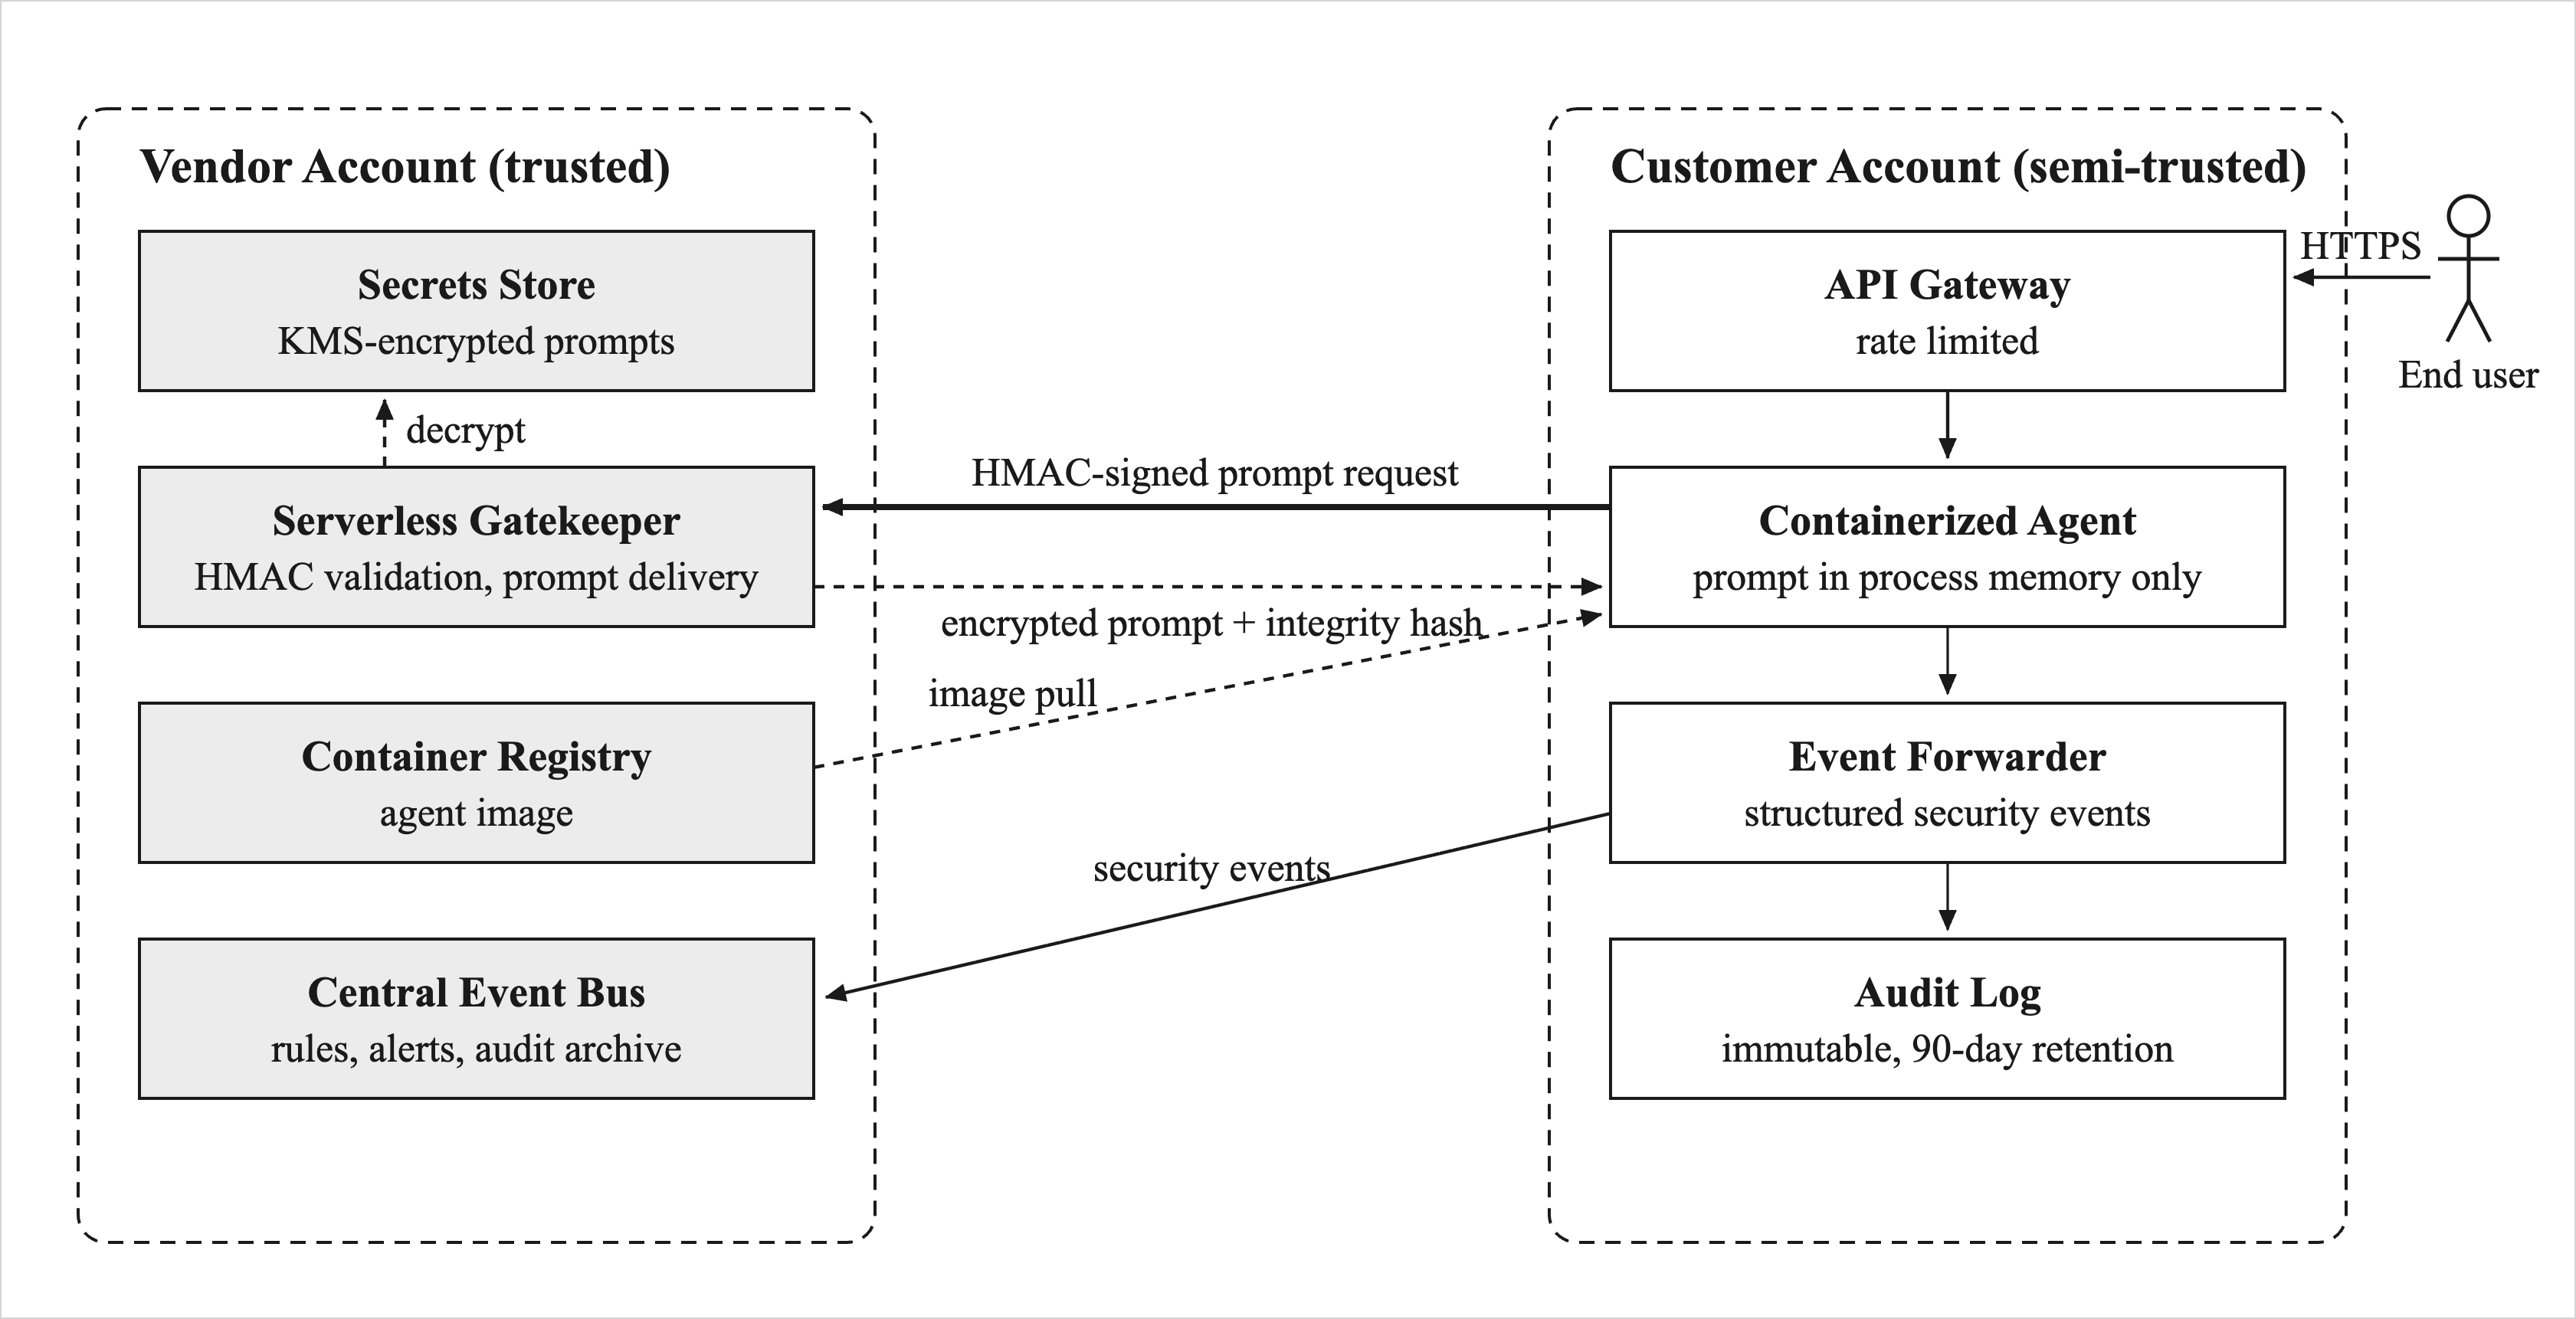
\includegraphics[width=\textwidth]{figA-two-account-architecture.png}
\caption{\label{fig:architecture}Two-account architecture for cross-domain prompt protection.}
\end{figure*}

The \emph{Vendor Account} contains the trusted components: a secrets store whose prompts are encrypted with a Key Management Service (KMS) key, a serverless gatekeeper in charge of authentication and prompt delivery, a container registry, and a central event bus. The \emph{Customer Account} contains the deployed components: the containerized agent, an API gateway with rate limiting, and an event-forwarding mechanism. The agent obtains its prompt at runtime and keeps it exclusively in process memory. This separation enforces an invariant on which the whole design depends: the system prompt is never persisted in customer-controlled storage and exists only transiently during inference.

Figure~\ref{fig:architecture} describes where components are deployed; the security of the architecture also depends on how requests are processed across them. Preserving prompt confidentiality across accounts requires a sequence of coordinated defenses applied at different stages of the interaction. Figure~\ref{fig:pipeline} shows this defense-in-depth pipeline as four sequential layers whose composition covers the complete request lifecycle.

\begin{figure*}[t]
\centering
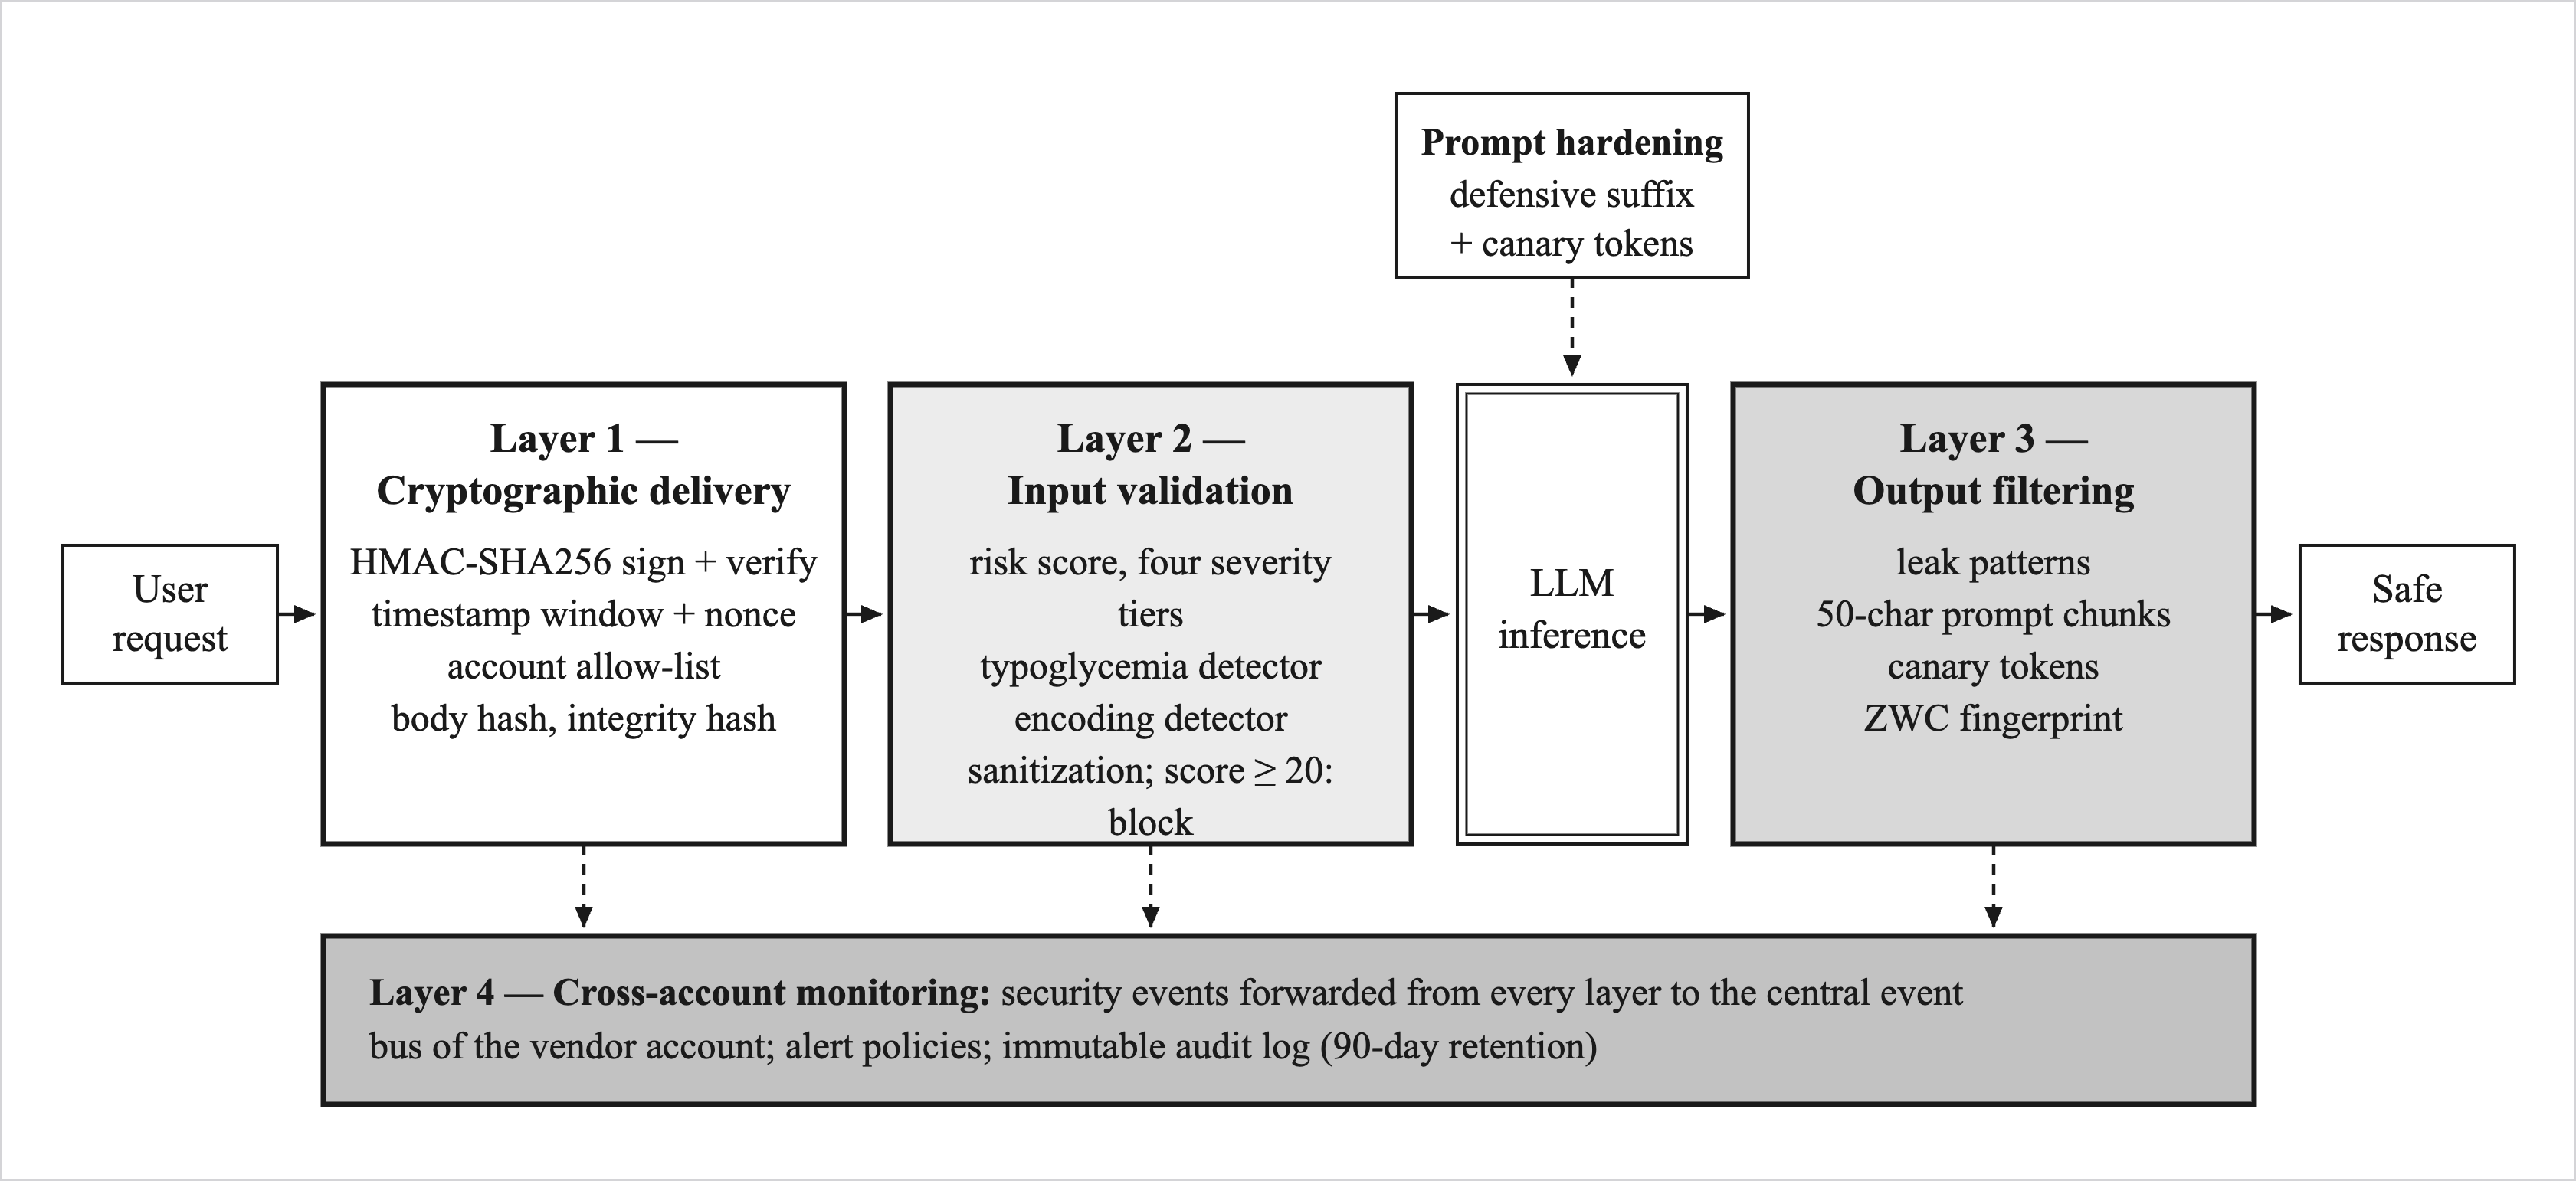
\includegraphics[width=\textwidth]{figB-defense-in-depth-pipeline.png}
\caption{\label{fig:pipeline}Defense-in-depth pipeline: Layers~1 and~2 act before model inference, Layer~3 acts on the model output, and Layer~4 receives the security events of every layer.}
\end{figure*}

Each layer covers a distinct part of the attack surface. Layer~1 secures prompt delivery through cryptographic request validation. Layer~2 applies OWASP-aligned input validation to detect adversarial inputs before they reach the model. Layer~3 filters model outputs and embeds forensic fingerprints to prevent leakage and support attribution. Layer~4 centralizes cross-account monitoring to enable anomaly detection and coordinated response. Figure~\ref{fig:layers} details the internal mechanism of each layer; the following subsections describe them in turn, followed by the prompt-level hardening that complements them.

\begin{figure*}[t]
\centering
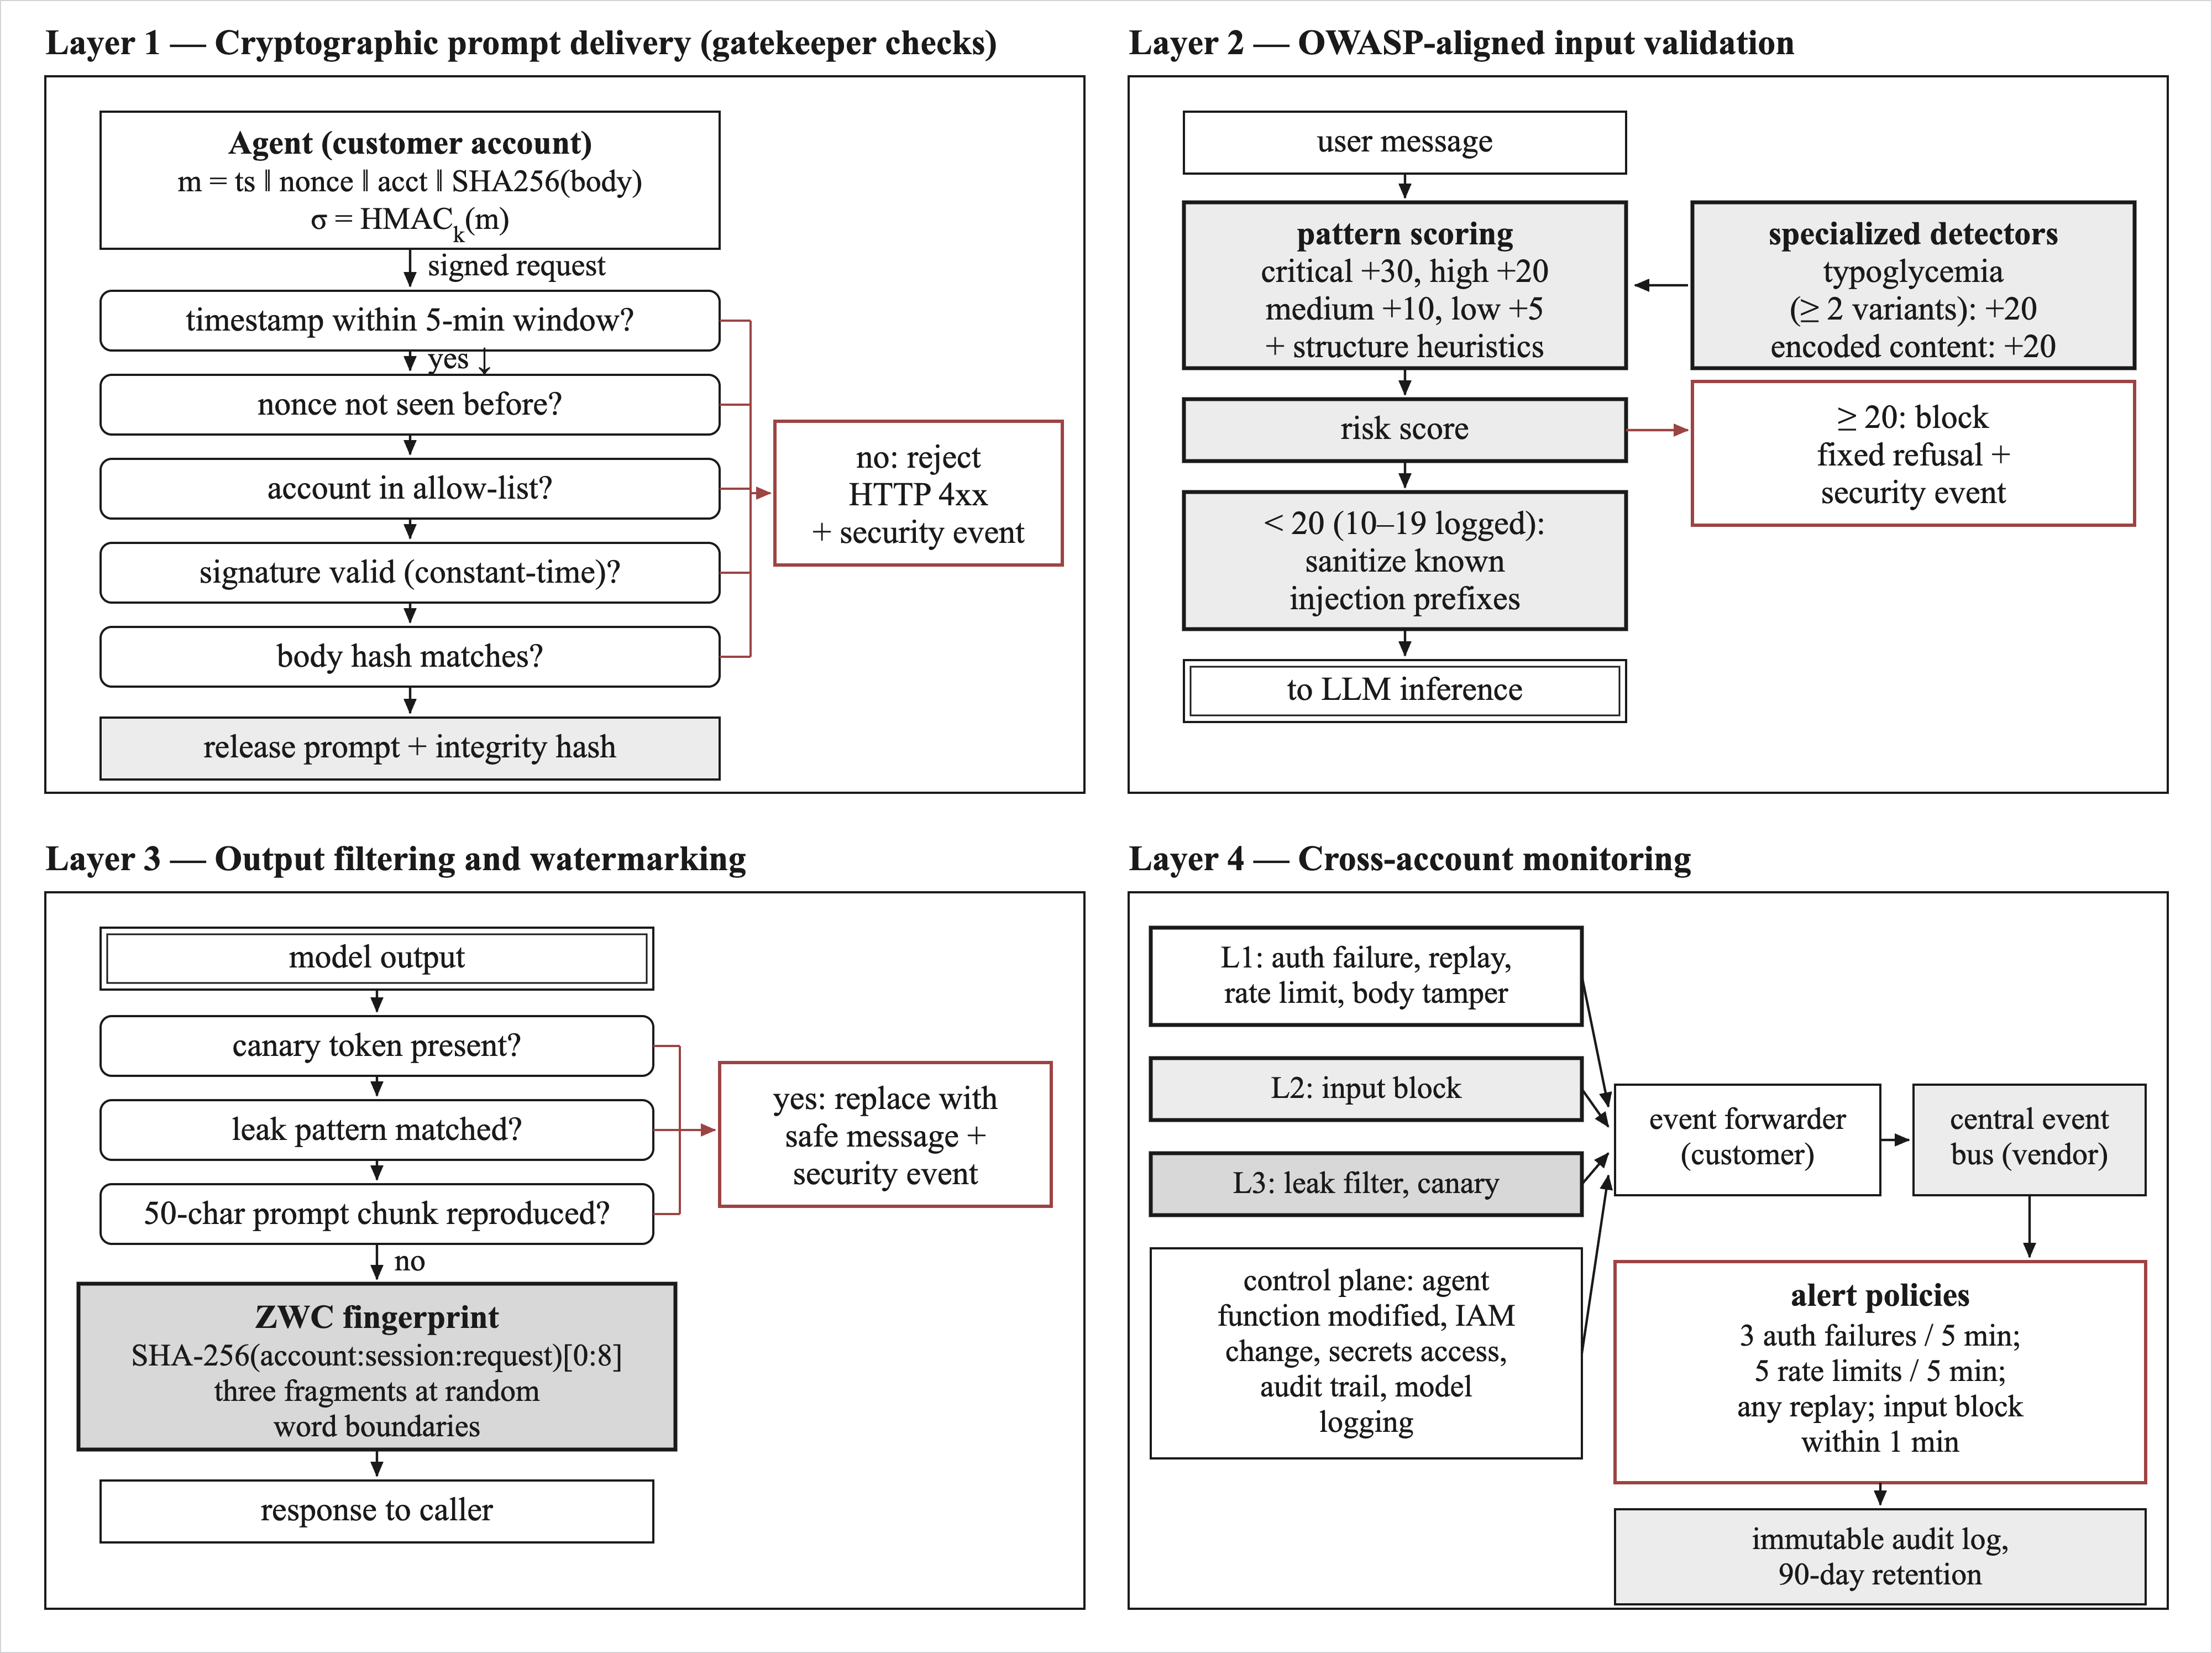
\includegraphics[width=\textwidth]{figC-internal-mechanism-layers.png}
\caption{\label{fig:layers}Internal mechanism of each defense layer as implemented in the reference implementation: validation order of the gatekeeper (Layer~1), scoring and blocking decision (Layer~2), output checks and fingerprint embedding (Layer~3), and event sources, forwarding, alerting, and audit (Layer~4).}
\end{figure*}

\subsection{Layer 1: Cryptographic Prompt Delivery}
\label{sec:layer1}

This layer guarantees that only authenticated agents can retrieve prompts and that requests can be neither tampered with nor replayed. The guarantee follows from a cryptographic binding between the request payload, the originating account, and temporal information. Each request carries an HMAC with SHA-256 (HMAC-SHA256) signature over a structured message:
\begin{equation}
\label{eq:hmac}
m = \mathit{ts} \;\|\; \mathit{nonce} \;\|\; \mathit{account\_id} \;\|\; \text{SHA256}(\mathit{body})
\end{equation}
The signature is $\sigma = \text{HMAC-SHA256}(k, m)$, where $k$ is a pre-shared secret key. The construction protects the integrity of the request body, binds the request to one account, and provides freshness through the timestamp and the nonce.

Before releasing the prompt, the gatekeeper checks four properties: (1)~the timestamp lies within a bounded window, set to five minutes in the reference implementation, which limits replay; (2)~the nonce has not been observed before, which a short-lived cache enforces within that window; (3)~the account identifier belongs to an allow-list; and (4)~the request body matches the signed hash. All comparisons use constant-time operations to avoid timing side channels. The gatekeeper additionally enforces a per-account request rate and raises an alert after repeated failed attempts from the same account. Together with the prompt, it returns an integrity hash (SHA-256 of the prompt content) that the agent verifies on receipt, which extends integrity protection end to end. The signing key is supplied at container build time through a build secret that is never written to an image layer, so it cannot be recovered from the image history.

At the application layer, the mechanism therefore provides request authenticity, payload integrity, and replay protection. These properties keep prompt delivery secure even against adversaries with visibility into the execution environment.

\subsection{Layer 2: OWASP-Aligned Input Validation}
\label{sec:layer2}

This layer mitigates prompt injection and adversarial manipulation by screening user inputs before they reach the model. It relies on a quantitative risk assessment aligned with the OWASP LLM Top~10~\cite{owasp2025} and with the complementary taxonomy of the National Institute of Standards and Technology (NIST)~\cite{nist2025aml,promptinjection2026}.

Every incoming message receives a risk score computed from the patterns it matches. The patterns correspond to known attack strategies, such as instruction override, jailbreak personas, prompt extraction requests, and structural injection markers, and are grouped into four severity tiers with additive weights: critical ($+30$), high ($+20$), medium ($+10$), and low ($+5$). Structural heuristics add smaller increments for unusually long inputs, an excessive number of line breaks, or embedded markup tags. Inputs whose score reaches a fixed threshold, set to 20, are blocked with a fixed refusal message; inputs in the medium band are logged as suspicious and allowed through. The threshold follows from the weights: a score of 20 corresponds to one high-severity pattern or to two independent medium-severity signals, so a single reference to an encoding scheme is tolerated while combinations of weaker signals trigger blocking. This design prevents explicit attacks without over-restricting legitimate technical queries; the empirical support for the operating point is reported in Section~\ref{sec:live}.

Two specialized detectors extend coverage beyond explicit patterns. A typoglycemia detector matches deliberately misspelled variants of security-critical keywords, such as ``ignroe'' or ``systme'', against a dictionary of known variants; two or more variants add $+20$ to the score. An encoding detector flags payloads hidden through base64, hexadecimal, or Unicode escape sequences, as well as explicit requests to decode ROT13 or similar transformations; any detected encoding adds $+20$. Before the message is forwarded to the model, a sanitization step replaces known injection prefixes, such as override commands or fake role markers, with a neutral placeholder. Together, these mechanisms form the first line of defense against adversarial inputs: they reduce the likelihood that malicious instructions reach the model while preserving flexibility for legitimate use.

\subsection{Layer 3: Output Filtering and Watermarking}
\label{sec:layer3}

This layer prevents the disclosure of sensitive information in model responses and enables forensic attribution of generated content. It processes every response with three complementary mechanisms: leakage detection, active signaling, and covert fingerprinting.

First, responses are inspected for prompt leakage with a set of compiled regular expressions that recognize meta-instructions, role definitions, jailbreak success indicators, and configuration dumps, and with a sliding-window comparison against the delivered prompt: the prompt is divided into 50-character chunks, and a response that reproduces any chunk is treated as a leak. Responses that trigger either check are replaced by a fixed safe message. Second, canary tokens are embedded in the prompt itself. Each canary is an HTML comment that contains a truncated SHA-256 hash derived from the account identifier and a timestamp; it is placed before and after the prompt body, remains invisible in normal operation, and produces an alert and a blocked response whenever it appears in an output. Third, every response is augmented with a steganographic fingerprint built from zero-width Unicode characters (ZWC)~\cite{zheng2020zwc,waterfall2024}. The fingerprint encodes a hash of the account, session, and request identifiers and is distributed across the generated text, so that it remains imperceptible and resists naive removal. Algorithm~\ref{alg:watermark} shows the embedding procedure of the reference implementation. The same module provides Personally Identifiable Information (PII) detection and redaction routines, which the static test suite exercises.

\begin{algorithm}[ht]
\caption{ZWC-based watermark embedding}
\label{alg:watermark}
\begin{algorithmic}[1]
\Function{Watermark}{$text, account, session, request$}
    \State $h \gets \text{SHA256}(account \| session \| request)$
    \State $w \gets \text{EncodeZWC}(h[0{:}8])$ \Comment{hex digits to ZWC sequences}
    \State $(w_1, w_2, w_3) \gets \text{Split}(w, 3)$
    \State $words \gets \text{SplitWords}(text)$
    \If{$|words| > 4$}
        \State $P \gets$ three distinct random positions in $[1, |words|)$
        \For{$(p_i, w_i)$ \textbf{in} $\text{zip}(\text{sorted}(P), (w_1, w_2, w_3))$}
            \State $words[p_i] \gets w_i \| words[p_i]$
        \EndFor
        \State \Return $\text{JoinWords}(words)$
    \Else
        \State \Return $w \| text$
    \EndIf
\EndFunction
\end{algorithmic}
\end{algorithm}

The mechanisms of this layer provide two complementary guarantees: prevention of prompt leakage at generation time, and post hoc attribution when content is exfiltrated. Proactive filtering and reactive traceability thus reinforce each other.

\subsection{Layer 4: Cross-Account Monitoring}
\label{sec:layer4}

This layer provides system-wide observability and coordinated detection of security events across the trust boundary. Monitoring is centralized in the vendor-controlled environment, so adversaries operating inside the customer account cannot suppress or alter security-relevant signals.

Events generated by all layers are forwarded to a central event bus, where they are aggregated and correlated. They include authentication failures, replay attempts, body-hash mismatches, and rate-limit violations from Layer~1; input-validation triggers from Layer~2; and leakage or canary detections from Layer~3. The customer account additionally forwards control-plane events that indicate tampering by a privileged principal, such as modifications of the agent function, changes to the IAM roles that protect it, direct access attempts to the secrets store, alterations of the audit trail, or activation of model-invocation logging. Alerting policies escalate suspicious activity: in the reference implementation, three gatekeeper authentication failures within five minutes, five rate-limit rejections within five minutes, or any replay attempt raise an alert, and every input-validation block in the customer account is forwarded within one minute. All events are also written to an immutable audit log with a 90-day retention period, so that incidents can be reconstructed even after a partial compromise.

This final layer complements the preceding ones with detection, accountability, and coordinated response across administrative domains.

\subsection{Prompt-Level Hardening}
\label{sec:hardening}

Besides the four layers, the prompt delivered by the gatekeeper is hardened in memory before the agent is instantiated. In addition to the canary tokens of Layer~3, a defensive suffix appends eight explicit rules that instruct the model never to reveal, paraphrase, or encode its instructions, to decline extraction attempts framed as roleplay, hypotheticals, or translation, and to answer such attempts with a fixed refusal sentence. This control is inexpensive and requires no infrastructure, but its effect depends entirely on the instruction-following behavior of the underlying model, which the architecture does not control. For that reason it is not counted as a defense layer: it is treated as an explicit factor in the multi-model evaluation and in the ablation study, and the reproducibility environment provides alternative variants of the suffix designed for small open-weight models (Section~\ref{sec:local-env}).

\section{Reference Implementation and Reproducibility}
\label{sec:implementation}

The implementation is a central part of the contribution: it shows that the architecture can be built from standard managed services, and it provides the artifacts used in every experiment reported in this article. The reference implementation and the experimental artifacts are publicly available\footnote{\url{https://github.com/dpetrocelli/defense-in-depth-agent-ip}}.

\subsection{Cloud Deployment}

The system is built on serverless services, which provide automatic scaling and cost-efficient operation, and is defined entirely as Infrastructure-as-Code (IaC) with Terraform. Two environments correspond to the two accounts of the model. The central environment provisions the vendor-side components: the encrypted secrets store and its KMS key, the gatekeeper function behind an HTTP endpoint, the container registry, the central event bus with its rules, the alerting topics, and the audit storage. The client environment provisions the customer-side components: the agent function packaged as a container image, the API gateway with throttling, the event forwarder, and the detection rules described in Section~\ref{sec:layer4}. The architecture relies only on service primitives that all major providers offer; Table~\ref{tab:mapping} lists the AWS services of the reference implementation and their equivalents on Azure and Google Cloud.

\begin{table*}[t]
\caption{\label{tab:mapping}Architectural components, services used in the reference implementation, and equivalent services on other providers.}
\centering
\footnotesize
\setlength{\tabcolsep}{4pt}
\begin{tabular}{@{}llll@{}}
\toprule
\textbf{Component} & \textbf{AWS (reference)} & \textbf{Azure} & \textbf{Google Cloud} \\
\midrule
Secrets store + KMS        & Secrets Manager + KMS            & Key Vault + Managed HSM          & Secret Manager + Cloud KMS \\
Serverless gatekeeper      & Lambda + API Gateway             & Functions + API Management       & Cloud Functions (2nd gen) \\
Container registry         & ECR                              & Container Registry               & Artifact Registry \\
Cross-account event bus    & EventBridge                      & Event Grid                       & Eventarc \\
Containerized agent (FaaS) & Lambda (container image)         & Functions (container)            & Cloud Run (container) \\
Immutable audit log        & S3 Object Lock + CloudWatch Logs & Immutable Blob Storage + Monitor & Cloud Logging + retention \\
\bottomrule
\end{tabular}
\end{table*}

The agent is a Python application that exposes an HTTP interface with three endpoints, for health checks, tool listing, and invocation, and runs both as a serverless function and as a local process. It is built on an agent framework with tool calling and ships with four demonstration tools (arithmetic, current time, string utilities, and Fibonacci numbers), which makes the injection surface realistic. In the cloud deployment the model is Amazon Nova Lite, invoked through the provider's managed inference service. Layer~1 is split between the gatekeeper function in the vendor account and a signing client inside the agent; Layers~2 and~3 are implemented as a self-contained filtering module inside the agent; Layer~4 combines the event forwarder, the event-bus rules, and the alarms of both accounts.

Deployment proceeds in three phases. In the \emph{build} phase, the container image is produced with the signing key mounted as a build secret, so that the key is available while the image is built but absent from every image layer. In the \emph{provisioning} phase, the customer-side resources are instantiated through cross-account access policies that allow the customer function to pull the image from the vendor registry without granting that permission to the customer administrator. In the \emph{activation} phase, the agent retrieves its prompt from the gatekeeper over the authenticated channel, verifies the integrity hash, applies the hardening of Section~\ref{sec:hardening}, and keeps the result only in process memory. Before serving traffic, a fail-closed pre-flight check verifies that model-invocation logging is disabled in the customer account, which enforces trust assumption~(4) of Section~\ref{sec:threats}.

\subsection{Security Configuration}

Every defense mechanism is governed by a feature flag exposed as an environment variable of the agent (Table~\ref{tab:flags}). All flags default to enabled, and disabling one of them changes only the corresponding mechanism, which allows layer configurations to be compared without code changes. The input sanitization step and canary detection are not governed by flags and remain active in every configuration. This configuration surface is the basis of the ablation study of Section~\ref{sec:ablation}.

\begin{table}[ht]
\caption{\label{tab:flags}Feature flags of the reference implementation and the mechanism each one governs.}
\centering
\scriptsize
\setlength{\tabcolsep}{2pt}
\begin{tabular}{@{}ll@{}}
\toprule
\textbf{Flag} & \textbf{Mechanism governed} \\
\midrule
\texttt{USE\_GATEKEEPER}          & L1: prompt retrieval through the gatekeeper \\
\texttt{ENABLE\_INPUT\_VALIDATION} & L2: risk scoring and specialized detectors \\
\texttt{BLOCK\_HIGH\_RISK\_INPUTS} & L2: blocking of high and critical inputs \\
\texttt{ENABLE\_RESPONSE\_FILTER}  & L3: leakage detection on model outputs \\
\texttt{ENABLE\_WATERMARKING}      & L3: ZWC fingerprint embedding \\
\texttt{ENABLE\_PREFLIGHT\_CHECK}  & Pre-flight model-logging check \\
\bottomrule
\end{tabular}
\end{table}

\subsection{Local Reproducibility Environment}
\label{sec:local-env}

To allow experimentation without cloud accounts, the repository provides a Docker Compose environment that combines LocalStack for cloud-service emulation and Ollama for local LLM inference. A single-account variant runs the agent against an emulated secrets store with the gatekeeper disabled. A multi-account variant reproduces the two-account model with two isolated LocalStack instances: a central instance hosts the gatekeeper function behind an API endpoint, the secrets store, the KMS key, and an alerting topic with a queue that allows Layer~4 alerts to be verified; a client instance provides a separate identity for the agent. The gatekeeper executes the same code as in the cloud deployment, so all four layers are exercised end to end without code modifications.

The model is selected through a configuration variable, and any model served by Ollama can be used. The agent uses the native Ollama driver of the agent framework, which transmits the system prompt and the tool definitions as separate fields of the request; an earlier configuration based on a generic proxy library silently dropped the system message when tools were present, which nullified the prompt-level hardening. The environment also provides three alternative defensive suffixes, a minimal variant, a variant that states an explicit boundary between protected and normal requests, and an example-based variant, designed for small open-weight models that either ignore the production suffix or over-apply it. Mechanisms that depend on model behavior, in particular the defensive suffix and the model's own refusals, remain sensitive to the underlying LLM, which is precisely what the multi-model evaluation measures. The repository also contains the experimental tooling: the static penetration-test suite, the attack and legitimate-query corpus with its runner, the false-positive corpus, and the latency benchmark.

\section{Experimental Methodology}
\label{sec:methodology}

\subsection{Metrics, Corpus, and Environments}
\label{sec:corpus}

Security effectiveness is measured on two levels. Controlled penetration testing verifies each mechanism against a fixed suite of 63 test cases in 12 categories aligned with the OWASP LLM Top~10~\cite{owasp2025} and the NIST taxonomy of adversarial machine learning~\cite{nist2025aml}; every test specifies attack vector, targeted goal, expected layer, payload, and pass/fail criterion. Live evaluation submits a corpus of 42 attack queries in eight categories of increasing sophistication, naive extraction (8), instruction override (5), jailbreak and persona change (7), encoded payloads (4), typoglycemia (4), social engineering (5), indirect injection through fake system markers (4), and multi-turn escalation (5), together with 23 legitimate queries in three length groups (10 short, 10 medium, 3 long), to a deployed agent. It measures the \emph{block rate}, the share of attack queries that do not obtain a substantive answer, the \emph{false-positive rate} (FPR), the share of legitimate queries that are blocked, and, in the new experiments, the \emph{attack success rate} (ASR), the share of attack queries whose final response leaks protected content, so that blocking and leakage are measured separately. In the live evaluation of Section~\ref{sec:live}, an attack counts as blocked when the request is rejected, the response is empty, or the response is a refusal; the new experiments refine this criterion with the per-request classification of Section~\ref{sec:multimodel-protocol}. Performance overhead is measured as per-layer latency at the 50th, 95th, and 99th percentiles (P50, P95, P99) and as throughput under load; deployability as monthly infrastructure cost on three providers. Two environments are used: the two-account AWS deployment of Section~\ref{sec:implementation}, with Amazon Nova Lite as the underlying model, for the live evaluation, the performance measurements, and the cost analysis; and the multi-account Docker Compose stack of Section~\ref{sec:local-env}, which runs the same agent and gatekeeper code against open-weight models served by Ollama, for the multi-model evaluation and the ablation study. Both use the test prompts of the corpus rather than a production prompt.

\subsection{Multi-Model Evaluation Protocol}
\label{sec:multimodel-protocol}

The multi-model evaluation answers RQ1 by holding every element of the pipeline fixed and varying only the underlying LLM, so that differences in outcome can be attributed to the model. Nine models from six families are evaluated, covering both deployment modes of the architecture. Amazon Nova Lite (\texttt{amazon.nova-lite-v1:0}) is invoked through Amazon Bedrock and serves as the reference model of the live evaluation. The eight open-weight models are served by Ollama 0.33.3 in the local environment, with the quantization published under each identifier: Llama~3.2 1B (\texttt{llama3.2:1b}, Q8\_0), Llama~3 8B (\texttt{llama3:8b}, Q4\_0), Gemma~3 4B (\texttt{gemma3:4b}), Gemma~4 E4B (\texttt{gemma4:e4b}, 4B effective parameters), Phi-4 Mini (\texttt{phi4-mini}, 3.8B), Mistral~7B (\texttt{mistral:7b}), Qwen~3.5 4B (\texttt{qwen3.5:4b}), and Qwen~3.5 9B (\texttt{qwen3.5:9b}, 9.6B), the last six at Q4\_K\_M; seven of them ran on a single laptop GPU (RTX 4060, 8~GB) and Gemma~4 E4B on an RTX 3090. All models run the same agent and gatekeeper code, and serving conditions are constant within each model, which is what the comparison across configurations requires.

The following factors are fixed across models. The base system prompt is the medium-length prompt of the corpus (about 600 characters), whose closing sentence is a minimal confidentiality instruction that forms part of the base prompt in every configuration; it is hardened with the production defensive suffix and the canary tokens of Section~\ref{sec:hardening}. The four demonstration tools were registered for all models except Gemma~3 4B and Llama~3 8B, whose runs were executed without tool registration. Decoding is deterministic (temperature 0, nucleus sampling disabled, at most 1,024 output tokens on Ollama). All four layers are enabled, which corresponds to configuration C4 of Table~\ref{tab:ablation-configs}. Every query is submitted in a fresh conversation, except the multi-turn escalation category, whose five queries form one session and are submitted in their listed order. Each model is evaluated in three independent runs, reported as mean and standard deviation. Requests that end in a transport error or a timeout are counted as errors and excluded from the denominators; the complete campaign comprises 10,530 requests, 7 of which ended in errors.

The outcome of every request is classified by the mechanism that determined it: \emph{L2 block} (risk score at or above the threshold), \emph{model refusal} (the model declines before any filtering), \emph{L3 filter} (the response filter replaced the output), \emph{canary} (a canary token appeared in the output), \emph{pass} (a substantive response reached the caller), or \emph{error}. Because Layer~2 blocks, canary detections, and model refusals return the same refusal sentence, the label is recorded by the agent as a structured audit field rather than inferred from the response text; the raw model output produced before Layer~3 is recorded as well. Leakage is assessed offline with the same criterion that Layer~3 applies at runtime: a response leaks if it contains a canary token or reproduces any 50-character chunk of the base prompt, ignoring case. The oracle is applied both to the final response, which yields the ASR, and to the raw model output, which yields the \emph{pre-filter leakage} of the model. The block rate is the share of attack queries whose outcome is an L2 block, a model refusal, an L3 filter, or a canary detection; the FPR is the share of legitimate queries with any of these outcomes. Results are reported per model, with the attribution of outcomes to mechanisms (Table~\ref{tab:multimodel-overall}), and per attack category (Table~\ref{tab:multimodel-percategory}).

\subsection{Defense-Layer Ablation Protocol}
\label{sec:ablation-protocol}

\begin{table*}[t]
\caption{\label{tab:ablation-configs}Ablation configurations. Layer~1 (gatekeeper delivery) and Layer~4 (monitoring) remain active in every configuration, since they do not act on the input--output path of a request; they are verified separately (Table~\ref{tab:l1-l4-verification}). DP denotes the defensive suffix of Section~\ref{sec:hardening}.}
\centering
\footnotesize
\setlength{\tabcolsep}{3pt}
\begin{tabular}{@{}llccccccc@{}}
\toprule
\textbf{Config.} & \textbf{Description} & \textbf{DP} & \textbf{L2 scoring} & \textbf{L2 blocking} & \textbf{Sanitization} & \textbf{L3 filter} & \textbf{Canary} & \textbf{Watermark} \\
\midrule
C0            & No defenses (model-only floor)             & --         & --         & --         & --         & --         & --         & -- \\
C1            & DP only                                    & \checkmark & --         & --         & --         & --         & --         & -- \\
C2            & DP + Layer~2                               & \checkmark & \checkmark & \checkmark & \checkmark & --         & --         & -- \\
C3            & DP + Layer~3                               & \checkmark & --         & --         & --         & \checkmark & \checkmark & \checkmark \\
C4            & DP + Layer~2 + Layer~3 (deployed pipeline) & \checkmark & \checkmark & \checkmark & \checkmark & \checkmark & \checkmark & \checkmark \\
C4$^{\dagger}$ & As C4 with Layer~2 in detect-only mode    & \checkmark & \checkmark & --         & \checkmark & \checkmark & \checkmark & \checkmark \\
\bottomrule
\end{tabular}
\end{table*}


The ablation study answers RQ2 by measuring how the security outcome changes when individual defenses are removed. The layers are not interchangeable classifiers: Layer~1 governs authentication, request integrity, account binding, and replay protection, and Layer~4 governs monitoring, auditability, and coordinated response; neither acts on the content of a request or a response, so removing them does not change the outcome of the attack corpus. Both are kept active in every configuration and verified separately, with attack cases of their own, in Table~\ref{tab:l1-l4-verification}. The ablation therefore varies the \emph{content-path protections}, the mechanisms that act on the input--output path of a request: the defensive suffix, Layer~2, and Layer~3. Layer~1 and Layer~4 are validated functionally rather than as factors of the ablation.

Table~\ref{tab:ablation-configs} summarizes the configurations. C0 disables every content defense and measures the floor set by the model itself, since the base prompt retains only its closing confidentiality sentence; C1 adds the defensive suffix alone; C2 and C3 add Layer~2 and Layer~3, respectively, on top of the suffix; C4 is the deployed pipeline and coincides with the condition of the multi-model evaluation; and C4$^{\dagger}$ keeps the pipeline of C4 but runs Layer~2 in detect-only mode, in which the risk score is computed and recorded while blocking is disabled, so that every attack reaches the model and Layer~3 and the verdicts of both layers are observed on the same request. Input sanitization and canary detection follow the Layer~2 and Layer~3 settings, respectively. All configurations are evaluated for the nine models with the fixed factors, repetitions, classification, and metrics of Section~\ref{sec:multimodel-protocol}. The contribution of a mechanism is the change in block rate and ASR between configurations that differ only in that mechanism: the defensive suffix from C0 to C1, Layer~2 from C1 to C2 and from C3 to C4, and Layer~3 from C1 to C3 and from C2 to C4. Complementarity is measured on C4$^{\dagger}$ by labeling each attack query with the verdict of Layer~2 (would block or pass) and with its downstream outcome (intercepted by Layer~3 or by a canary, refused by the model, or passed), which yields Table~\ref{tab:complementarity}; queries that pass Layer~2 and are intercepted by Layer~3 are the direct evidence of complementarity, and queries that pass both are evaluated with the leakage oracle.

Layer~1 is verified with deterministic cases executed against the gatekeeper of the multi-account environment, which runs the production code: a valid signed request must return the prompt with a valid integrity hash, and each violated property must produce the response that follows from the validation order of the gatekeeper without disclosing prompt content. Layer~4 is verified by triggering each event class: the gatekeeper-side classes (repeated authentication failures, replay, rate limiting) in the same environment, whose alert topic is read through a subscribed queue, and the agent-side classes (Layer~2 blocks, Layer~3 filters, canary detections) and the customer-side control-plane rule on the two-account cloud deployment, where delivery is read from the archive log of the central event bus and from the invocation metrics of the forwarding rules, because the alarms of Layer~4 are cloud metric alarms that the local environment does not emulate.

\section{Security Evaluation}
\label{sec:security-eval}

\subsection{Controlled Penetration Testing}
\label{sec:pentest}

All 63 test cases of the controlled suite passed: 44 input-side tests (direct and multi-turn extraction, jailbreak and ``Do Anything Now'' (DAN) personas, instruction override, prompt injection, encoding and typoglycemia evasion, social engineering), 15 output-side tests (output leakage, Personally Identifiable Information (PII) exfiltration, response safety), and 4 replay and authentication bypass tests, which were rejected with Hypertext Transfer Protocol (HTTP)~403 responses that disclosed no information. The typoglycemia detector blocked obfuscated variants that defeat a naive regular-expression approach, the sliding-window comparison of Layer~3 detected partial leakage of fragments of 50 or more characters that the pattern-based check alone did not capture, and eight boundary-condition tests confirmed that attacks crafted to lower their Layer~2 score were still mitigated by Layer~3.

\subsection{Live Two-Account Deployment}
\label{sec:live}

To validate the architecture under realistic conditions, the full four-layer stack was deployed across two separate cloud accounts, vendor and customer, and exposed to the 42 attack queries and the 23 legitimate queries of Section~\ref{sec:corpus}. Table~\ref{tab:live_detection} reports the outcome per category: every category was fully blocked except naive extraction (6 of 8) and multi-turn escalation (3 of 5), for a total of 38 of 42 attacks (90.5\%) and no false positive on the 23 legitimate queries. The four queries that were not blocked are reconnaissance probes that obtain no prompt content.

\begin{table}[tb]
\caption{\label{tab:live_detection}Live deployment: attack detection by category (42 attacks, 23 legitimate queries). FP = false positive.}
\centering
\scriptsize
\setlength{\tabcolsep}{3pt}
\begin{tabular}{@{}lccl@{}}
\toprule
\textbf{Attack category} & \textbf{Blocked} & \textbf{Rate} & \textbf{Defense} \\
\midrule
Override commands     & 5/5   & 100\% & L2 (risk score) \\
Jailbreak / DAN       & 7/7   & 100\% & L2 (risk score) \\
Encoded payloads      & 4/4   & 100\% & L2 (encoding det.) \\
Typoglycemia          & 4/4   & 100\% & L2 (typo det.) \\
Social engineering    & 5/5   & 100\% & L2+L3 \\
Indirect injection    & 4/4   & 100\% & L2 (structural) \\
Naive extraction      & 6/8   &  75\% & L2+L3+defensive prompt \\
Multi-turn            & 3/5   &  60\% & L2+L3 (escalation) \\
\midrule
\textbf{Total attacks}   & \textbf{38/42} & \textbf{90.5\%} & \\
\textbf{Legitimate (FP)} & \textbf{0/23}  & \textbf{0.0\%}  & \\
\bottomrule
\end{tabular}
\end{table} Multi-turn escalation has the lowest rate because input validation is stateless: escalation sessions spread their intent over turns that are individually benign, only one of the five sessions contains a turn that reaches the blocking threshold by itself, and the sessions that were blocked were intercepted by the escalation heuristics of Layer~2 and the output-side filter of Layer~3 once the responses approached protected content; cumulative session-level scoring would close this gap. A sensitivity analysis over the corpus supports the operating point of Layer~2: the coverage of the score-based detector is stable between thresholds 15 and 20 (20 of 42 attacks) and falls sharply at 25 (12 of 42), while no legitimate query scores above 5. The detector set was calibrated iteratively against a preliminary live run, which raised the overall blocking rate from 59.5\% to the final 90.5\% while keeping false positives at zero. Under concurrent load, throughput remained stable up to 50 concurrent requests (13.8 requests per second) and degraded at higher concurrency because of infrastructure limits.

\subsection{Multi-Model Evaluation}
\label{sec:multimodel}

\begin{table}[ht]
\caption{\label{tab:multimodel-overall}Multi-model evaluation with the full pipeline (configuration C4): blocked attacks, block rate, attack success rate (ASR, leaked final responses), false positives (FP) on the 23 legitimate queries, and false-positive rate (FPR). Mean $\pm$ standard deviation over three runs; requests that ended in transport errors or timeouts are excluded from the denominators.}
\centering
\scriptsize
\setlength{\tabcolsep}{2.5pt}
\begin{tabular}{@{}lccccc@{}}
\toprule
\textbf{Model} & \textbf{Blocked} & \textbf{Block rate} & \textbf{ASR} & \textbf{FP} & \textbf{FPR} \\
               & (n/42)           & (\%)                & (\%)         & (n/23)      & (\%) \\
\midrule
Nova Lite    & \TBD & \TBD & \TBD & \TBD & \TBD \\
Llama 3.2 1B & \TBD & \TBD & \TBD & \TBD & \TBD \\
Llama 3 8B   & \TBD & \TBD & \TBD & \TBD & \TBD \\
Gemma 3 4B   & \TBD & \TBD & \TBD & \TBD & \TBD \\
Gemma 4 E4B  & \TBD & \TBD & \TBD & \TBD & \TBD \\
Phi-4 Mini   & \TBD & \TBD & \TBD & \TBD & \TBD \\
Mistral 7B   & \TBD & \TBD & \TBD & \TBD & \TBD \\
Qwen 3.5 4B  & \TBD & \TBD & \TBD & \TBD & \TBD \\
Qwen 3.5 9B  & \TBD & \TBD & \TBD & \TBD & \TBD \\
\bottomrule
\end{tabular}
\end{table}

\begin{table*}[t]
\caption{\label{tab:multimodel-percategory}Block rate per attack category and model with the full pipeline (configuration C4), as blocked/total over the three runs.}
\centering
\scriptsize
\setlength{\tabcolsep}{3pt}
\begin{tabular}{@{}lccccccccc@{}}
\toprule
\textbf{Attack category} & \textbf{Nova} & \textbf{Llama} & \textbf{Llama} & \textbf{Gemma} & \textbf{Gemma} & \textbf{Phi-4} & \textbf{Mistral} & \textbf{Qwen} & \textbf{Qwen} \\
 & \textbf{Lite} & \textbf{3.2 1B} & \textbf{3 8B} & \textbf{3 4B} & \textbf{4 E4B} & \textbf{Mini} & \textbf{7B} & \textbf{3.5 4B} & \textbf{3.5 9B} \\
\midrule
Naive extraction (8)      & \TBD & \TBD & \TBD & \TBD & \TBD & \TBD & \TBD & \TBD & \TBD \\
Override commands (5)     & \TBD & \TBD & \TBD & \TBD & \TBD & \TBD & \TBD & \TBD & \TBD \\
Jailbreak / DAN (7)       & \TBD & \TBD & \TBD & \TBD & \TBD & \TBD & \TBD & \TBD & \TBD \\
Encoded payloads (4)      & \TBD & \TBD & \TBD & \TBD & \TBD & \TBD & \TBD & \TBD & \TBD \\
Typoglycemia (4)          & \TBD & \TBD & \TBD & \TBD & \TBD & \TBD & \TBD & \TBD & \TBD \\
Social engineering (5)    & \TBD & \TBD & \TBD & \TBD & \TBD & \TBD & \TBD & \TBD & \TBD \\
Indirect injection (4)    & \TBD & \TBD & \TBD & \TBD & \TBD & \TBD & \TBD & \TBD & \TBD \\
Multi-turn escalation (5) & \TBD & \TBD & \TBD & \TBD & \TBD & \TBD & \TBD & \TBD & \TBD \\
\midrule
\textbf{Total (42)}       & \TBD & \TBD & \TBD & \TBD & \TBD & \TBD & \TBD & \TBD & \TBD \\
\bottomrule
\end{tabular}
\end{table*}


Table~\ref{tab:multimodel-overall} reports the full pipeline across the nine models under the protocol of Section~\ref{sec:multimodel-protocol}; since the corpus, the prompt, the hardening, the decoding parameters, and the four layers are identical for every model, the variation across rows is attributable to the underlying LLM.

No final response met the verbatim leakage criterion: the ASR is 0.0\% for all nine models, that is, none of the 1,134 attack requests of this condition returned a canary token or a 50-character chunk of the base prompt to the caller. The block rate, in contrast, depends strongly on the model: it ranges from 62.7\% for Llama~3.2 1B to 93.7\% for Nova Lite, with Mistral~7B, Gemma~4 E4B, Llama~3 8B, and Qwen~3.5 9B above 84\% and Phi-4 Mini and Qwen~3.5 4B below 75\%. The value of Nova Lite is consistent with the 90.5\% of the live deployment. Standard deviations across runs do not exceed 4.1 points, so the differences between models are not run-to-run variation.

The attribution columns separate the model-independent part of this result from the model-dependent part. Layer~2 blocked exactly 75 of the 126 attack requests of every model, that is, 25 of the 42 attacks in each run (59.5\%): the risk scorer and the specialized detectors are deterministic, so their contribution does not depend on the model, and it coincides with the 59.5\% floor observed during the calibration of Section~\ref{sec:live}. Everything above that floor comes from the refusals of the model, which follow the defensive suffix, and from Layer~3. Refusals account for 43 of the remaining 51 requests for Nova Lite and for none of them for Llama~3.2 1B, with the other models in between (13 to 33); Layer~3 intercepted between 0 and 7 responses per model. The requests that were neither blocked nor refused, from 8 for Nova Lite to 47 for Llama~3.2 1B, were answered without reproducing protected content. Two caveats apply: a refusal is recognized by the fixed refusal sentence, so a model that declines in its own words counts as having passed, and passing without leak is judged by the verbatim oracle.

Table~\ref{tab:multimodel-percategory} shows where the model matters. Four of the eight naive extraction attacks, four of the five override commands, four of the seven jailbreaks, three of the four encoded payloads, two of the four typoglycemia variants, four of the five social-engineering attacks, three of the four indirect injections, and one of the five multi-turn turns reach the blocking threshold of Layer~2 on their own; this floor is visible in the column of Llama~3.2 1B, which coincides with it in every category except multi-turn escalation, where Layer~3 adds four interceptions. The remaining attacks are intercepted only when the model refuses them or Layer~3 filters the response: naive extraction and typoglycemia are fully covered by four models each, whereas multi-turn escalation remains the weakest category for every model except Llama~3 8B (from 3 of 15 turns for Gemma~3 4B and Phi-4 Mini to 15 of 15), although every escalation session was intercepted in at least one turn for all nine models.

The false-positive rate is also model-dependent, and it originates in the defensive suffix rather than in Layer~2, which blocked no legitimate query in any configuration of the campaign. Five models answered between one and four of the 23 legitimate queries with the fixed refusal sentence, mostly short generic questions such as ``What time is it?'', which yields FPRs between 4.3\% (Llama~3 8B) and 15.9\% (Gemma~3 4B); Llama~3.2 1B and the two Qwen models produced no false positive. The 11.6\% of Gemma~4 E4B is of a different nature: the model returned empty responses to the three long legitimate queries, which the classification counts as refusals, also without any defense (C0), so this rate reflects the model runtime rather than the defenses. Finally, the pre-filter leakage shows what Layer~3 removed: with the full pipeline, 29.4\% of the raw outputs that reached the model reproduced a chunk of the prompt for Mistral~7B, 5.9\% for Llama~3.2 1B, Llama~3 8B, and Gemma~4 E4B, and 3.9\% for Qwen~3.5 4B, and none of these fragments reached the caller.

In answer to RQ1, the architecture kept the attack success rate, as measured by the verbatim criterion, at zero for every model family, while the block rate, which measures how early an attack is stopped, varied by 31 points between the weakest and the strongest model; the variation is entirely attributable to the defensive suffix and the refusal behavior of the model, since the contribution of Layer~2 was identical for all models.

\subsection{Defense-Layer Ablation Study}
\label{sec:ablation}

\begin{table*}[t]
\caption{\label{tab:ablation-results}Ablation results per configuration and model: block rate (BR, \%), attack success rate (ASR, \%), and false-positive rate (FPR, \%). Mean over three runs; standard deviations are reported in the repository.}
\centering
\scriptsize
\setlength{\tabcolsep}{3pt}
\begin{tabular}{@{}llcccccccccc@{}}
\toprule
\textbf{Config.} & \textbf{Metric} & \textbf{Nova} & \textbf{Llama} & \textbf{Llama} & \textbf{Gemma} & \textbf{Gemma} & \textbf{Phi-4} & \textbf{Mistral} & \textbf{Qwen} & \textbf{Qwen} & \textbf{Mean} \\
 & & \textbf{Lite} & \textbf{3.2 1B} & \textbf{3 8B} & \textbf{3 4B} & \textbf{4 E4B} & \textbf{Mini} & \textbf{7B} & \textbf{3.5 4B} & \textbf{3.5 9B} & \\
\midrule
C0 & BR & 0.0 & 0.0 & 0.0 & 0.0 & 0.0 & 0.0 & 0.0 & 0.0 & 0.0 & 0.0 \\
 & ASR & 15.9 & 3.2 & 34.1 & 23.8 & 2.4 & 4.0 & 23.8 & 9.5 & 0.0 & 13.0 \\
 & FPR & 0.0 & 0.0 & 0.0 & 0.0 & 13.0 & 0.0 & 0.0 & 0.0 & 0.0 & 1.4 \\
\midrule
C1 & BR & 93.6 & 6.3 & 50.0 & 50.0 & 79.4 & 42.9 & 71.4 & 23.8 & 77.8 & 55.0 \\
 & ASR & 0.0 & 1.6 & 7.1 & 0.0 & 1.6 & 0.0 & 19.0 & 15.9 & 1.6 & 5.2 \\
 & FPR & 13.0 & 2.9 & 4.3 & 4.3 & 11.6 & 13.0 & 4.3 & 0.0 & 0.0 & 6.0 \\
\midrule
C2 & BR & 93.7 & 60.3 & 85.7 & 81.0 & 78.6 & 76.2 & 85.7 & 65.9 & 84.1 & 79.0 \\
 & ASR & 0.8 & 1.6 & 0.0 & 0.0 & 2.4 & 0.0 & 12.7 & 1.6 & 0.0 & 2.1 \\
 & FPR & 11.6 & 1.4 & 4.3 & 0.0 & 11.6 & 13.0 & 4.3 & 0.0 & 0.0 & 5.2 \\
\midrule
C3 & BR & 92.1 & 8.7 & 54.8 & 50.0 & 73.8 & 42.9 & 78.6 & 40.5 & 78.6 & 57.8 \\
 & ASR & 0.0 & 0.0 & 0.0 & 0.0 & 0.0 & 0.0 & 0.0 & 0.0 & 0.0 & 0.0 \\
 & FPR & 4.3 & 0.0 & 4.3 & 2.9 & 8.7 & 13.0 & 8.7 & 0.0 & 4.3 & 5.2 \\
\midrule
C4 & BR & 93.7 & 62.7 & 85.7 & 81.0 & 88.1 & 73.8 & 89.7 & 69.8 & 84.9 & 81.0 \\
 & ASR & 0.0 & 0.0 & 0.0 & 0.0 & 0.0 & 0.0 & 0.0 & 0.0 & 0.0 & 0.0 \\
 & FPR & 7.2 & 0.0 & 4.3 & 15.9 & 11.6 & 13.0 & 13.0 & 0.0 & 0.0 & 7.2 \\
\bottomrule
\end{tabular}
\end{table*}

\begin{table*}[t]
\caption{\label{tab:complementarity}Complementarity between Layer~2 and Layer~3 (configuration C4$^{\dagger}$, Layer~2 in detect-only mode): number of attack queries by Layer~2 verdict and downstream outcome, summed over the three runs. ``L3 intercepts'' includes canary detections; ``passes'' reports the number of leaked responses in parentheses.}
\centering
\scriptsize
\setlength{\tabcolsep}{4pt}
\begin{tabular}{@{}lcccccc@{}}
\toprule
 & \multicolumn{3}{c}{\textbf{Layer~2 would block}} & \multicolumn{3}{c}{\textbf{Layer~2 passes}} \\
\cmidrule(lr){2-4} \cmidrule(lr){5-7}
\textbf{Model} & \textbf{L3 intercepts} & \textbf{Model refuses} & \textbf{Passes (leak)} & \textbf{L3 intercepts} & \textbf{Model refuses} & \textbf{Passes (leak)} \\
\midrule
Nova Lite    & \TBD & \TBD & \TBD & \TBD & \TBD & \TBD \\
Llama 3.2 1B & \TBD & \TBD & \TBD & \TBD & \TBD & \TBD \\
Llama 3 8B   & \TBD & \TBD & \TBD & \TBD & \TBD & \TBD \\
Gemma 3 4B   & \TBD & \TBD & \TBD & \TBD & \TBD & \TBD \\
Gemma 4 E4B  & \TBD & \TBD & \TBD & \TBD & \TBD & \TBD \\
Phi-4 Mini   & \TBD & \TBD & \TBD & \TBD & \TBD & \TBD \\
Mistral 7B   & \TBD & \TBD & \TBD & \TBD & \TBD & \TBD \\
Qwen 3.5 4B  & \TBD & \TBD & \TBD & \TBD & \TBD & \TBD \\
Qwen 3.5 9B  & \TBD & \TBD & \TBD & \TBD & \TBD & \TBD \\
\bottomrule
\end{tabular}
\end{table*}

\begin{table*}[t]
\caption{\label{tab:l1-l4-verification}Verification of Layer~1 and Layer~4. The Layer~1 cases and the gatekeeper-side Layer~4 cases were executed against the gatekeeper of the multi-account environment, which runs the production code; the agent-side Layer~4 cases were executed against the two-account cloud deployment and read from the archive of the central event bus and the delivery metrics of its rules. Latencies are measured from the triggering request.}
\centering
\scriptsize
\setlength{\tabcolsep}{3pt}
\begin{tabular}{@{}lp{3.6cm}p{1cm}p{3.4cm}p{5.2cm}@{}}
\toprule
\textbf{Layer} & \textbf{Case} & \textbf{Adversary} & \textbf{Expected outcome} & \textbf{Observed} \\
\midrule
L1 & Valid signed request & -- & HTTP 200, prompt with valid integrity hash & HTTP 200; prompt returned; integrity hash verified \\
L1 & Missing headers; account not in allow-list; timestamp outside the 5-minute window; forged signature; tampered body & $\mathcal{A}_1$, $\mathcal{A}_2$ & HTTP 400 (headers) or 403, no prompt content & As expected in all five cases; body tampering produced its audit event \\
L1 & Replayed nonce & $\mathcal{A}_1$, $\mathcal{A}_2$ & HTTP 403, replay event & First use HTTP 200; replay HTTP 403 with replay audit event \\
L1 & Per-account rate limit exceeded & $\mathcal{A}_2$ & HTTP 429, rate-limit event & HTTP 429 with rate-limit audit event (60 requests per minute) \\
\midrule
L4 & Repeated authentication failures & $\mathcal{A}_1$ & Events on central bus; alert raised & Audit events on every failure; gatekeeper alert at the fifth failure (0.01\,s); no alert at the third, since the metric alarm with threshold~3 is not emulated locally \\
L4 & Replay attempt & $\mathcal{A}_1$, $\mathcal{A}_2$ & Event on central bus; immediate alert & Replay audit event; no alert locally (metric alarm not emulated) \\
L4 & Five rate-limit rejections within 5 min & $\mathcal{A}_2$ & Events on central bus; alert raised & Gatekeeper alert after the fifth rejection (0.01\,s) \\
L4 & Layer~2 input block & $\mathcal{A}_2$ & Event forwarded within 1 min & \texttt{PromptInjectionAttempt} on the central bus and alert published; 70\,s (60-s alarm period) \\
L4 & Layer~3 leakage filter & $\mathcal{A}_2$ & Event on central bus & \texttt{PromptLeakageDetected} on the central bus and alert published; 100\,s \\
L4 & Canary token in output & $\mathcal{A}_2$ & Event on central bus; alert raised & Not exercised: no canary token was reproduced in any run \\
L4 & Customer-side tampering (agent function modified) & $\mathcal{A}_1$ & Control-plane event forwarded & Alert published on the central topic 53\,s after the change (the rule targets the topic directly) \\
\bottomrule
\end{tabular}
\end{table*}


Table~\ref{tab:ablation-results} gives block rate, ASR, and FPR for every configuration of Table~\ref{tab:ablation-configs} and every model. Without content defenses (C0) no attack is blocked, and the intrinsic leakage of the models ranges from 0.0\% (Qwen~3.5 9B) to 34.1\% (Llama~3 8B), 13.0\% on average. The defensive suffix alone (C1) raises the mean block rate to 55.0\% and lowers the mean ASR to 5.2\%, but its effect is the most model-dependent of the study: the block rate goes from 6.3\% for Llama~3.2 1B to 93.6\% for Nova Lite, and Mistral~7B and Qwen~3.5 4B still leak in 19.0\% and 15.9\% of the attacks. Adding Layer~2 (C2) raises the mean block rate by 24.0 points. Layer~2 blocks the same 25 attacks per run for every model, so its gain is largest where the model refuses least: +54.0 points for Llama~3.2 1B, +42.1 for Qwen~3.5 4B, and between +31 and +36 for Gemma~3 4B, Phi-4 Mini, and Llama~3 8B, against +0.1 for Nova Lite and $-$0.8 for Gemma~4 E4B, whose refusals already cover most of what Layer~2 blocks. Layer~2 reduces the mean ASR to 2.1\% but does not eliminate it: Mistral~7B leaks in 12.7\% of the attacks and four other models in 0.8--2.4\%, because Layer~2 stops only the attacks that match its patterns and the model answers the rest. Adding Layer~3 instead (C3) raises the mean block rate by only 2.7 points, but it brings the ASR to 0.0\% for all nine models, as does the full pipeline (C4).

The two layers therefore contribute different properties: Layer~2 determines how many attacks are stopped before inference, at no cost in false positives; Layer~3 determines whether what the model generates reaches the caller, and it closes the residual leakage left by the model and by Layer~2. The marginal contributions summarize this asymmetry: +24.0 and +23.3 points of block rate for Layer~2 against +2.7 and +2.0 for Layer~3, and $-$5.2 and $-$2.1 points of ASR for Layer~3 against $-$3.1 and 0.0 for Layer~2. The false positives of the pipeline come from the defensive suffix (mean FPR 6.0\% in C1) and, marginally, from Layer~3, which filtered one legitimate response of Qwen~3.5 9B; Layer~2 added none.

Table~\ref{tab:complementarity} shows the two layers on the same requests. Of the 17 attack queries per run that pass Layer~2, Layer~3 intercepted the response for Qwen~3.5 4B (10 of 51 requests over the three runs), Mistral~7B (9), Llama~3.2 1B (3), and Nova Lite (2); for the other five models, the queries that passed Layer~2 were either refused by the model or answered without leaking. Layer~3 also intercepted responses to attacks that Layer~2 would have blocked (11 for Qwen~3.5 4B, 6 for Mistral~7B, 3 for Gemma~4 E4B), which is redundant coverage. No request passed both layers with a leaked response for any model: in detect-only mode the block rate falls to between 4.8\% (Llama~3.2 1B) and 95.9\% (Nova Lite), yet the ASR remains 0.0\%. The cells ``Layer~2 would block, passes'' quantify what the deterministic layer adds beyond the model: 72 of 75 such requests for Llama~3.2 1B, 48 for Qwen~3.5 4B, and 42 for Llama~3 8B, against none for Nova Lite, so for the weakest models Layer~2 is the only mechanism that keeps these attacks from reaching inference. For the cloud reference model the defensive suffix alone already intercepts 117 of the 126 attack requests, and multi-turn escalation is the only category that remains partially covered in every configuration (7 to 9 of 15 turns), consistent with the stateless scoring discussed in Section~\ref{sec:live}; the per-category ablation of every model is provided in the repository.

Table~\ref{tab:l1-l4-verification} reports the verification of the layers outside the ablation. All eight Layer~1 cases produced the expected response of the gatekeeper, without prompt content in any rejected case. For Layer~4, the gatekeeper-side alert on repeated failures fired at the fifth failure, which is the threshold implemented in the function, whereas the three-failure and replay alerts of the design are cloud metric alarms that the local environment does not emulate. On the cloud deployment, a Layer~2 block, a Layer~3 filter, and a configuration change of the agent function all reached the central bus or the alert topic within the one-minute evaluation period of the alarms; the canary case could not be exercised because no run reproduced a canary token. The verification also exposed a defect of the deployment: the policy of the central alert topic authorized the event rules to publish only on behalf of the customer accounts, so the alerts fanned out from the central bus were being denied; the policy was corrected, the table was measured after the correction, and the delivery metrics of the rules before and after it document the cause.

In answer to RQ2, the defense-in-depth claim holds in a specific form, and for the content-path protections: the defensive suffix supplies most of the block rate, but with an effect that depends on the model and is small for the smallest one; Layer~2 adds a model-independent floor of 59.5\% at no cost in false positives; and Layer~3 is the component that removes the residual verbatim leakage, measured with the same criterion the layer applies at runtime, so its value lies in what it had to remove, up to 29.4\% of the raw outputs, rather than in the zero itself. Layer~1 and Layer~4 are not factors of this comparison: they were validated functionally, as authentication and integrity controls and as the auditing and response path, respectively. No configuration without Layer~3 achieved zero leakage for all nine models, no configuration without Layer~2 exceeded a mean block rate of 58\%, and only the full pipeline combined a mean block rate above 80\% with zero leakage across models.

\section{Performance and Cost Evaluation}
\label{sec:perf-cost}

\begin{table}[tb]
\caption{\label{tab:perf-cost}Latency overhead per defense layer over $n=1{,}000$ requests (top) and incremental monthly cost of the software-only defense stack over a conventional agent deployment, at 50K requests and excluding model inference (bottom).}
\centering
\scriptsize
\setlength{\tabcolsep}{4pt}
\begin{tabular}{@{}lrrr@{}}
\toprule
\textbf{Layer} & \textbf{P50} & \textbf{P95} & \textbf{P99} \\
\midrule
L1: HMAC validation     & 2.1  & 3.8  & 5.2 \\
L2: Risk scoring        & 8.3  & 14.7 & 19.1 \\
L3: Output filter + ZWC & 12.5 & 22.3 & 31.6 \\
L4: Event forwarding    & 4.1  & 8.2  & 12.4 \\
\midrule
\textbf{Total (ms)}     & \textbf{27.0} & \textbf{49.0} & \textbf{68.3} \\
\bottomrule
\end{tabular}

\vspace{1.2em}

\setlength{\tabcolsep}{2.5pt}
\begin{tabular}{@{}llrrr@{}}
\toprule
\textbf{Component} & \textbf{Service primitive} & \textbf{AWS} & \textbf{Azure} & \textbf{GCP} \\
\midrule
Secrets + encryption & Managed secrets + KMS key     & \$1.40 & \$1.60 & \$1.06 \\
Gatekeeper + API     & FaaS function + HTTP endpoint & \$0.05 & \$0.00 & \$0.00 \\
Event bus            & Cross-account event routing   & \$0.00 & \$0.00 & \$0.00 \\
Audit storage        & Immutable logs (90-day)       & \$0.25 & \$0.25 & \$0.25 \\
Monitoring           & Log ingestion + retention     & \$0.03 & \$0.10 & \$0.05 \\
Container registry   & Image storage (\textasciitilde100\,MB) & \$0.01 & \$5.01 & \$0.01 \\
\midrule
\textbf{Total}       &                               & \textbf{\$1.74} & \textbf{\$6.96} & \textbf{\$1.37} \\
\bottomrule
\end{tabular}
\end{table}

\subsection{Latency Overhead}

The upper part of Table~\ref{tab:perf-cost} reports the latency added by each defense layer in the AWS reference implementation. The total overhead at P99 is 68.3\,ms, well under the 100--200\,ms range that is imperceptible in conversational applications. Cold starts of the container-based function average 1.2\,s; provisioned concurrency removes them at approximately \$4.50 per month and per instance, a cost that is not part of the base infrastructure cost reported next.

\subsection{Infrastructure Cost}

The lower part of Table~\ref{tab:perf-cost} reports the cost that the defense layers add to a conventional agent deployment on three cloud providers at 50,000 requests per month; Function-as-a-Service (FaaS) denotes the serverless execution of the gatekeeper. The figures are \emph{independent of model inference}, since the defenses operate at the transport and application layers and do not modify inference calls.

The economic value of the architecture is incremental: it adds security controls to a conventional cloud-native agent, at USD 1.37--6.96 per month across the evaluated providers, without dedicated hardware or a specialized inference runtime. This is not a claim of security equivalence with TEEs; it positions the architecture as a low-cost, deployable containment baseline when hardware-backed isolation is unavailable or disproportionate to the threat model.

\section{Discussion and Limitations}
\label{sec:discussion}

The multi-model evaluation and the ablation study qualify the defense-in-depth claim of the conference version in two ways. First, the effectiveness of the architecture is not uniform across models: the deterministic components, Layer~2 and Layer~3, behave identically for every model, but the prompt-level hardening, which supplies most of the block rate, depends on the instruction-following behavior of the LLM and ranges from negligible (Llama~3.2 1B) to almost complete (Nova Lite). Changing the underlying model therefore changes how early attacks are stopped, but not the leakage, which the output-side layer kept at zero for all nine models. Second, the layers are complementary in function rather than redundant in coverage: Layer~2 stops attacks before inference and never blocked a legitimate query, Layer~3 removes the residual leakage that the model and Layer~2 let through, and the false positives come from the defensive suffix, which several small models over-apply to short legitimate queries. These results argue for treating the defensive suffix as a tunable, model-specific component, and for keeping Layer~3 in every deployment regardless of the model.

From a systems perspective, the trust model exchanges hardware-backed guarantees for broader deployability. Its root of trust is a correctly configured cloud IAM, weaker than hardware attestation but available on every provider, and the defense-in-depth design mitigates this weakness: when one layer is compromised, for example through an IAM misconfiguration, the remaining layers continue to enforce protection. The architecture and TEE-based approaches are therefore complementary; recent measurements show TEE overheads below 10\% on CPUs and below 7\% on GPUs~\cite{teeperf2025}, so high-assurance deployments may combine both.

Several limitations remain. Rotating the HMAC signing key requires rebuilding the container image; risk-scoring thresholds may need tuning per deployment; text-processing pipelines that normalize Unicode may strip the zero-width watermark; adversarial fine-tuning on captured prompt--response pairs was not evaluated; and covert signaling mechanisms carry risks of their own~\cite{stegocollusion2024}. The adversarial evaluation is static: adaptive adversaries that refine their inputs from the observed blocking behavior were not evaluated, and runtime memory access lies outside the threat model of Section~\ref{sec:threats}. The new evaluations add limitations of their own. The leakage oracle detects the verbatim reproduction of 50-character chunks of the prompt and of canary tokens, the same criterion that Layer~3 applies, so a paraphrased disclosure of the instructions does not count as a leak and the outcomes classified as passed without leak must be read with this caveat, in particular for the small models that answered many attacks; an independent oracle applied to the recorded raw outputs is the natural next step. The classification of refusals relies on the fixed refusal sentence and on empty outputs, which undercounts models that decline in their own words and inflated the false-positive rate of one model whose runtime returned empty responses to long queries. The corpus is the 42-query corpus of the conference version, so each legitimate query moves the FPR by 4.3 points, and sampling-based decoding was not evaluated. The open-weight models were served at 4-bit or 8-bit quantization on a single GPU, and two of them without the demonstration tools registered, so absolute rates may differ under other serving conditions; the comparison across configurations is unaffected, since each model was evaluated under constant conditions.

From an ethical standpoint, the watermarking mechanism identifies accounts and sessions rather than individual users. Its use should be disclosed transparently and confined to intellectual property protection and forensic analysis, in line with standard privacy practices.

\section{Conclusions and Future Work}
\label{sec:conclusions}

This article addressed the protection of AI agent intellectual property in multi-tenant cloud deployments as a cross-domain trust problem and presented a defense-in-depth architecture for it. The composition of cryptographic prompt delivery, OWASP-aligned input validation, output filtering with steganographic watermarking, and cross-account monitoring into a sequential trust chain provides prompt confidentiality, output integrity, and forensic traceability with standard cloud services and without TEEs or specialized hardware. The architecture is cloud-agnostic; its serverless reference implementation, deployed across two separate accounts, showed strong security effectiveness against realistic attack scenarios, a low performance overhead, and a negligible infrastructure cost.

\TODO{Add the conclusions of the multi-model evaluation (RQ1) and of the defense-layer ablation study (RQ2) after the experimental results are available.}

Future work will extend the architecture in several directions: optional integration with TEE-based inference for high-assurance deployments, automated rotation of the HMAC signing key without downtime, formal verification of the security properties of the trust chain, and evaluation against adaptive adversaries. Further directions include redundant watermarking that combines ZWC steganography with token-based schemes~\cite{kirchenbauer2023watermark,synthid2024}, and stateful detection mechanisms for multi-turn interactions.


\begin{small}

\authorcontributions{
The authors confirm contribution to the paper as follows: DP: Conceptualization, Software, Investigation, Data curation, Validation, Writing -- review and editing; JMF: Conceptualization, Methodology, Formal analysis, Writing -- original draft, Writing -- review and editing. All authors reviewed the results and approved the final version of the manuscript.
}

\competinginterests{
The authors have declared that no competing interests exist.
}

\aideclaration{
During the preparation of this work, the authors used Claude (Anthropic) to assist with the drafting and editing of the manuscript and with the scripts that aggregate the experimental records. After using this tool, the authors reviewed and edited the content as needed and take full responsibility for the content of the publication.
}

\dataavailability{
The reference implementation, the reproducibility environment, the corpus, the experimental tooling, and the raw results are available at \url{https://github.com/dpetrocelli/defense-in-depth-agent-ip}.
}

\balance
\bibliography{references}

\end{small}

\vspace*{0pt}

\cornersize{.2}
\setlength{\fboxsep}{8pt}

% Please, don't remove the Citation Box (edited at the copyediting stage)
\ovalbox{
\begin{minipage}{\dimexpr\columnwidth-4\fboxsep-2\fboxrule\relax}
\textbf{Citation:} D. Petrocelli and J. M. Fern\'andez. \emph{Layered Prompt Protection for AI Agents in Customer-Controlled Cloud Accounts: Model Robustness and Defense-Layer Contribution}. Journal of Computer Science \& Technology, vol.~XX, no.~X, pp.~X--X, 2026.

\textbf{DOI:} to be assigned at the copyediting stage.

\textbf{Received:} to be completed. \textbf{Accepted:} to be completed.

\textbf{Copyright:} This article is distributed under the terms of the Creative Commons License CC-BY-NC-SA.
\end{minipage}
}

\end{document}
